%%%%%%%%%%%%%%%%%%%%%%%%%%%%%%%%%%%%%%%%%%%%%%%%%%%
% DOCUMENT CLASS DECLARATION
%%%%%%%%%%%%%%%%%%%%%%%%%%%%%%%%%%%%%%%%%%%%%%%%%%%
%% Use the following options:
% \documentclass[paper type% ("letterpaper" required)
% , one or two sided% ("oneside" or "twoside")%
% , font size% ("12pt" required)%
% , document type% ("these", "memoire", "memoireprojet" or "thesepararticles")%
% , document language ("francais" or "english)%
% , addition options% ("creativecommons" if the document is under the creative commons license, "hyperref", "withAlgo2e" to use algorithm2e package with proper formating)
%]{thETS}




%% Exemple with a Ph.D thesis under creative commons, using hyperref
\documentclass[letterpaper%
, twoside%
, 12pt%
,these%
, english%
,creativecommons,hyperref%
]{thETS}

\usepackage{siunitx}
\usepackage{tikz}
\usepackage{pgf}
\usepackage{mdwlist}
\usepackage{multirow}
\usepackage{booktabs}

%%%%%%%%%%%%%%%%%%%%%%%%%%%%%%%%%%%%%%%%%%%%%%%%%%%
% IMPORTANT: PRINTING WITH THE PROPER MARGINS
%%%%%%%%%%%%%%%%%%%%%%%%%%%%%%%%%%%%%%%%%%%%%%%%%%%
%% If you create a pdf with pdftex, and print it using acrobat reader, set the
%% "scaling" option to "none" to print with the proper margins.
%%%%%%%%%%%%%%%%%%%%%%%%%%%%%%%%%%%%%%%%%%%%%%%%%%%


%%%%%%%%%%%%%%%%%%%%%%%%%%%%%%%%%%%%%%%%%%%%%%%%%%%
% DECLARATION OF AN ADDITION LIST OF REFERENCES
%%%%%%%%%%%%%%%%%%%%%%%%%%%%%%%%%%%%%%%%%%%%%%%%%%%
%% Exemple of an additional list of references called "refs"
% "refs" is used as a suffix to all bibliography related commands
\newcites{refs}{LIST OF REFERENCES}

%%%%%%%%%%%%%%%%%%%%%%%%%%%%%%%%%%%%%%%%%%%%%%%%%%%
% TITLE PAGE OPTIONS
%%%%%%%%%%%%%%%%%%%%%%%%%%%%%%%%%%%%%%%%%%%%%%%%%%%

\title{METHODOLOGY AND ALGORITHMS FOR HIGH-LEVEL MODELLING OF COSMIC
RADIATION IMPACTS ON ELECTRICAL SYSTEMS}

\author{HASSAN ANWAR}
\authorcopyright{HASSAN ANWAR}

\datesoutenance{"20-December-2017"}

\datedepot{"02-December-2017"}

\directeur{M. }{Claude Thiebeault}{Départment de génie électrique  à l’École de technologie supérieure}

%\directeur{Mrs.}{Prénom Nom}{Nom du département et institution}

\codirecteur{Mrs.}{Yvon Savaria}{Départment de génie électrique  à l’École Polytechnique de Montréal}

%\codirecteurB{M.}{Prénom Nom}{département et institution}

\president{M.}{First Name Last Name}{Department and institution}

\examinexterne{M.}{First Name Last Name}{Department and institution}

%\jury{Mme.}{Prénom Nom}{département et institution}{}


%%%%%%%%%%%%%%%%%%%%%%%%%%%%%%%%%%%%%%%%%%%%%%%%%%%
% CHANGING THE NAME OF THE DIPLOMA
%%%%%%%%%%%%%%%%%%%%%%%%%%%%%%%%%%%%%%%%%%%%%%%%%%%
%% It is possible to change the name of the diploma by redefining
% the command \lediplome, as follows:
%\renewcommand{\lediplome}{OF A MASTER’S DEGREE\\WITH THESIS IN ELECTRICAL ENGINEERING\\M.A.Sc.}

\listfiles

%%%%%%%%%%%%%%%%%%%%%%%%%%%%%%%%%%%%%%%%%%%%%%%%%%%
% ACTUAL DOCUMENT
%%%%%%%%%%%%%%%%%%%%%%%%%%%%%%%%%%%%%%%%%%%%%%%%%%%
\begin{document}

\pagenumbering{Roman}

%%- Title page -%%
\maketitle

%%- Jury presentation -%%
\presentjury

%%- Foreword -%%
%\begin{foreword}
%
%\lipsum[1] % Texte de remplissage pour donner un exemple de la mise en page
%
%\end{foreword}



%%- Acknowledgements -%%
%\begin{acknowledgements}
%
%\lipsum[1] % Text filling, to have an example of the layout
%
%
%\end{acknowledgements}


%%- Summary -%%

%\begin{summary}{French title}{mot-clé1, mot-clé2}
%
%\lipsum[1] % Text filling, to have an example of the layout
%
%\end{summary}


%%- Abstract -%%





\begin{abstract}{FPGA, SEU, Modeling.}
Cosmic radiation   (CR)   produces soft errors in aircraft embedded electronic systems. Aircraft flying at an altitude of  55,000   feet,   and cross-polar routes   (North or   South latitudes)   are prone to neutron flux. CMOS based electronics are subject to hard and soft errors. Equipment protection against   CR   is becoming critical. The solutions to   protect electrical systems  
from cosmic rays are   developed but
unfortunately,   these solutions are costly,   time,   and energy consuming, e.g.,   dedicated heavy conductive electrical path. To progress towards the safe and efficient aircraft,   it is now necessary to anticipate the aircraft embedded system constraints in the early phase of the aircraft design. 
In this project,   we will   study the   novel algorithms   and methodology   for high levels modeling   of cosmic  
radiation impacts on   the aircraft. This thesis aims at defining a   novel approach for high-level modeling of digital sequential circuits.   In   particular,  our   thesis   intends   to   provide   solutions   able   to   mitigate   multiple   problems,  
including   a) Signature generations on the FPGA-based emulation platform, c) Analyze the signatures from the radiation-based experiment, d) Modelling the faulty behavior of the sequential circuit from the signatures observed at lower abstraction level to abstract it at the higher level of abstraction, and d)  Improved bits relative sensitivity difference based emulation strategy for FPGA based emulation platform. The methodology adopted in this thesis for modeling and analysis of the sequential circuits is based on the Hidden Markov Model (HMM). 
\end{abstract}

%%- Table of contents -%%
\tableofcontents
 
%%- List of tables -%%
\listoftables


%%- List of figures -%%
\listoffigures


%%- List of abbreviations -%%
\begin{listofabbr}[3cm]
\item [DUT]  Design Under Test 

\item [FPGA]  Field-Programmable Gate Array 
HDL Hardware Description Language 


\item [SBU] Single-Bit Upset 
\item [SEE] Single-Event Upset 
\item [SEL] Single-Event Latch-up 
\item [SER] Soft Error Rate 
\item [SET] Single-Event Transient 
\item [SEU] Single-Event Upset 
\item [SRAM] Static Random Access Memory 
\item [TMR] Triple Modular Redundancy 
\end{listofabbr}


%%%- List of symbols -%%
%\begin{listofsymbols}[3cm]
%\item [a] Première lettre de l'alphabet
%\item [A] Première lettre de l'alphabet en majuscule
%\end{listofsymbols}


\cleardoublepage

\pagenumbering{arabic}

% Marginpar to the left of the document
\reversemarginpar

%%%%%%%%%%%%%%%%%%%%%%%%%%%%%%%%%%%%%%%%%%%%%%%%%%%
% THESIS EXAMPLE
%%%%%%%%%%%%%%%%%%%%%%%%%%%%%%%%%%%%%%%%%%%%%%%%%%%

\chapter{Introduction}

%Prepare the tests on the EPICEA active sub-system (to be subcontracted)
%- Develop the active EPICEA sub-system for a SRAM-based CR emulation strategy for complex systems. Use
%of FPGA circuits from Xilinx allowing CR emulation (without CR illumination) by bit flipping for preparing
%the tests to be performed by the CR test subcontractor

\section{Context}
\label{introduction}

This thesis is part of a wider project, called EPICEA (Electromagnetic Platform for lightweight 
Integration/Installation of electrical systems in Composite Electrical Aircraft), in collaboration with several 
companies and agencies (Bombardier, Isoneo, ARTTIC, ONERA, AXESSIM, FOKKER ELMO BV, IDS). The EPICEA project will approach
numerous avionic engineering design issues in the advancement of future aircraft, aiming at a significant
reduction of energy consumption through more electrical aircraft and systems integration. The EPICEA project strives to understand the electromagnetic (EM) issues on composite electric aircraft (CEA). This includes the analysis
and characterization of EM coupling, interconnects, and cosmic radiations (CR) on electrical systems together
with new concepts of antennas design to maintain performance in a composite environment without modifying
aircraft aerodynamics.

This thesis contribution to the EPICEA project is "the study of CR effects on aircraft electrical systems based on the reconfigurable fabric, e.g., Field Programmable Field array (FPGA)." This work focuses on the extraction of the faulty response (signature) from the sequential digital circuit implemented on an FPGA-based platform. This extraction will be performed to help investigate the effects of CR on an embedded electronic system of the aircraft and to model and analyze the faulty behavior of the sequential digital circuits. This thesis aims at developing the high-level fault model that will use to investigate the effects of radiation on the aircraft flying at the altitude of 50,000 feet or above. 

\section{Problem Statement}

A soft error will occur when a radiation event causes enough charge disturbance to flip the state of a logic gate, memory element, or flip-flop. The soft errors are also referred as radiation-induced faults, e.g., neutrons from the cosmic rays. The fault caused by the SEUs have implications on the behavior of the system. However, the soft errors do not break the silicon but can corrupt the underlying functionality and produce severe consequences if they are successfully propagated to the primary outputs or stored by the memory cell. In this work, we will evaluate the faulty behaviors of the sequential circuit, given the faulty sequential circuit behavior, and model it to the high-level of abstraction. We want to make the high-level fault model to see the severity of the faulty behavior induced by the SEUs.



This thesis helps to find; at high altitude when aircraft gets more exposure to the radiation the reliability of the FPGA based embedded systems is a primary concern; the phenomena causing faults in the FPGA based embedded systems should be studied in a way to know early in the embedded electronic design of the aircraft if mitigation strategies are required to deal this higher radiation level. 

In order to accomplish our tasks, we need to understand the space radiation environment which has two preliminary sources --- galactic cosmic radiation and solar energetic particles~\cite{SWE20216}. The galactic cosmic radiation from outside the solar system consists mostly of energetic protons and heavy ions, e.g., iron. Solar energetic particles are commonly associated with the solar flare events and primarily dominated by the proton.  The space radiation is an unavoidable space weather phenomena. This research thesis is solely concern with the aircraft flying at the altitude of 50,000 feet or above, where the vulnerability of the circuit is due to the neutrons~\cite{xilinnseu}. The cosmic rays are originating in outer space and travel at nearly the speed of light and strike the earth from all directions. These cosmic radiations are ranging from lightest to heaviest elements in the periodic table. When these high-energy cosmic rays interact with the earth's magnetosphere, neutrons are generated, often referred to as an air shower~\cite{lesea2005rosetta}.  An intense neutron environment exists at higher altitudes in the atmosphere, 10 km to 40 km.  Long-haul aircraft are flying at the altitudes of 50,000 feet nearly 15 km at the latitude of \ang{60} under the influence of greatest neutron flux approximately 500 times that a ground-based observer in Newyork City~\cite{lesea2005rosetta}. When these neutrons interact with the semiconductor, e.g., silicon they can produce secondary particles if these secondary particles are charged and they can generate the trails of an electron-hole pair of a few microns in length and if this trail happens near the PN-junction in a transistor, a voltage spike can generate. This voltage spike is enough to change the state of a memory cell or flip-flop, results in a drastic consequence and cause Single Event Upsets (SEUs) also called soft-error in SRAM-based FPGAs. The impact and implications of the soft-errors due to the interaction of neutrons with the avionics embedded system are now recognized as an area of active research. Especially, the incident happened with the Qantas Flight Airbus A330-303 flying from Singapore to Perth went under the two terrifying dives due to the malfunction of the on-flight computer. After, the investigation it revealed that high-energy particles from the outer space --- were the responsible for the malfunction of the computer. And, the potential triggering event was the single-event effect (SEE) interacting with one of the integrated circuits (ICs) within the CPU module. 




%
%The Neutrons are generated in the atmosphere when cosmic rays in the outer space, strike Earth from all the direction. When these neutrons interact with the semiconductor e.g., silicon they can generate secondary particles, if these secondary particles are charged and they are able to generate the trails of electron-hole pair of a few microns in length and if this trail happens near the PN-junction in a transistor, a voltage spike can generate. This voltage spike is enough to change the state of a memory or flip-flop.

Therefore, fault management strategies are essential to apply on the aircraft's embedded systems. Before need to know to apply the mitigation techniques early in the embedded electronic design, if we know the high-level fault model of the FPGA-based circuits at high-level of abstraction that facilitate without going into the detailed simulation get the faulty behavior of the component at high-level.

  




%\begin{figure}
% \centering
%  \captionsetup{justification=centering}    
%   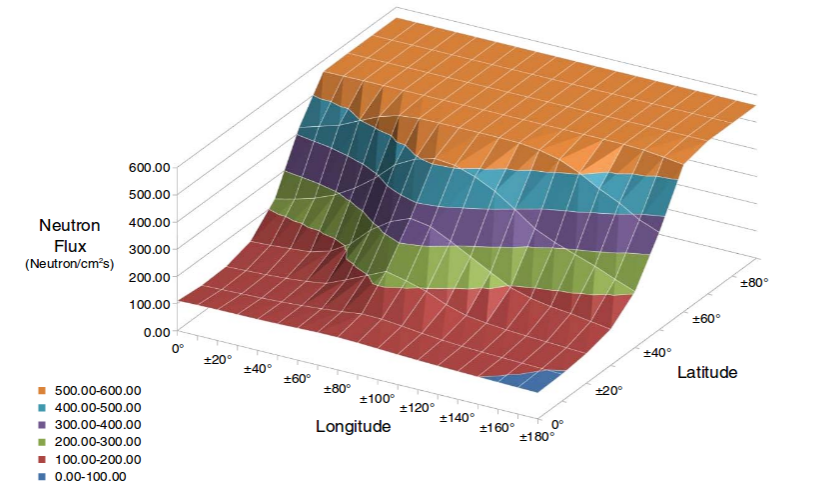
\includegraphics[scale=0.4]{figures/img/neutron-flux.png}
%   \caption{Neutron Flux at 40,000 Feet.}
%\label{fig:neu-flux}
%\end{figure}





\section{Research Objectives}


The main objective this thesis --- is to develop a methodology for modeling the faulty sequential circuits to model the output of the soft error problem at a behavioral level. We plan to use the high-level modeling techniques, e.g., Hidden Markov Model, to model the faulty behavior of the sequential circuits. The faulty behavior model will be based on analytical expressions, the signature (circuit fault response),derived from  experimental data generate by performing fault emulation on the FPGA. In this work, a novel approach will be introduced to analyze the fault origination and propagation in the case of faulty sequential circuits, and will allow developing new models that can accurately be used to estimate the severity of the faulty behavior from the signatures of the faulty circuits. The objectives of the present Ph.D. thesis are explained below: 

\begin{itemize}


\item{The objective of this thesis is to develop a faulty behavior model
at a high-level of abstraction. 


\item The objective of the thesis is to construct a model from the faulty response observed at low-level circuit fault emulation.

\item{Develop a library of the faulty behavior model of the sequential circuit
components comprising a Simulink model. So, each time designers need to analyze potential faulty behavior of a circuit at a high-level of abstraction, designer can utilize the faulty components from the library}.

\item The sub-objective of developing a behavioral fault model of a circuit is to generate a library of faulty components reusable at high-level of abstraction}.



\item{The model has the capability (a feature) to produce the faulty output of a circuit, and the probability of occurrence of faults.}

\item The purpose of this model is to find the severity of a faulty behavior of the sequential circuit. 

\item The model is used for the signature analysis for the sequential circuit.






%
%\item{The developed models could be used to
%replace any component of the entire circuit with faulty versions of the components described
%at a high-level of abstraction. The purpose of doing so to ensure that the effect of faulty behavior of each
%component on a system could be analyzed at a high-level of abstraction and the mitigation
%technique could be used to improve the robustness of critical parts of the design.}
%
%
%\item{The model will have the capability to compute the signature, also provide the worst-case input test vector, which has the highest probability to generate the faulty output, for any given sequential circuit. The model for sequential logic will have the ability to measure the maximum and average signature probabilities to construct a novel probabilistic model.}
%
%\item{Develop an abstraction of hardware signature that can be integrated into the high-level model, e.g., Simulink models.}
%
%\item{The goal of this research is to develop an approach for modeling the faulty behavior of a
%digital sequential circuit in the presence of the fault injection. The concept behind the fault injection process is to accelerate the occurrences of the signatures in the system to evaluate its functional behavior under the influence of expected faults on the
%FPGA-based systems.}





\end{itemize}




\subsection{Challenges}
Inorder to to achieve the above mentioned objectives. The main challenges we foresee are:
\begin{itemize}

\item Make a model at higher-level of abstraction from the data extracted at a lower level that represent the behavioral model of the respective signatures.
\item Develop a flow to convert faulty behavioral response of a sequential circuit into respective high-level model. This flow will be extensively validated by the fault emulation on FPGA. Develop a  fault behavioral model of different sequential circuits, e.g., counter, and FIR filter.

\item Develop a relationship between the bit-flip and the fault-model.

\end{itemize}


  

\section{Contribution}


This research thesis proposes a fault behavior model with the modeling techniques, e.g., Markovian-analysis in a novel way (utilize hidden Markov model (HMM) to represent faulty behavior of the sequential circuits). The Markovian system analysis will use to synthesize the faulty output of a circuit at high-level of abstraction. The existing faulty behavior model of the sequential circuits are not accurate as mostly models were based on simulation and on fault occurrence assumption. 

The previous work on soft error analysis and evaluation were focused on the circuit level. Most of the work done based on the interaction of the cosmic rays with the silicon atoms and its analysis, prediction of error, estimating the model of transistors and circuit layout structure that can tolerate radiations effects. On circuit level researchers were more focused on the generation and propagation of the radiation-induced transient pulses. The effects of these pulses are simulated with the help of SPICE. These fundamental analyses are essential and provide insight of soft error rate. However, they can not take the overall erroneous behavior of the circuit at the architecture level --- the errors produced at the low level propagate to the high level of abstraction. Further, the increased complexity of integrated circuits, and integration of several components, it is more difficult now to do the low-level circuit analysis and make the model at low-level. It is a more viable solution to find the faulty response of the circuit at the low level and model it to the high-level of abstraction. The high-level design suppresses a lot of unnecessary details, reduce the complexity, and its closer to the designer way of thinking. Our problem is unique in terms that it involve emulation at the circuit level and behavioral modeling as well, as can be depicted from the Figure~\ref{fig:ychart}.


\begin{figure}[tb!]

 \centering
  \captionsetup{justification=centering}    
   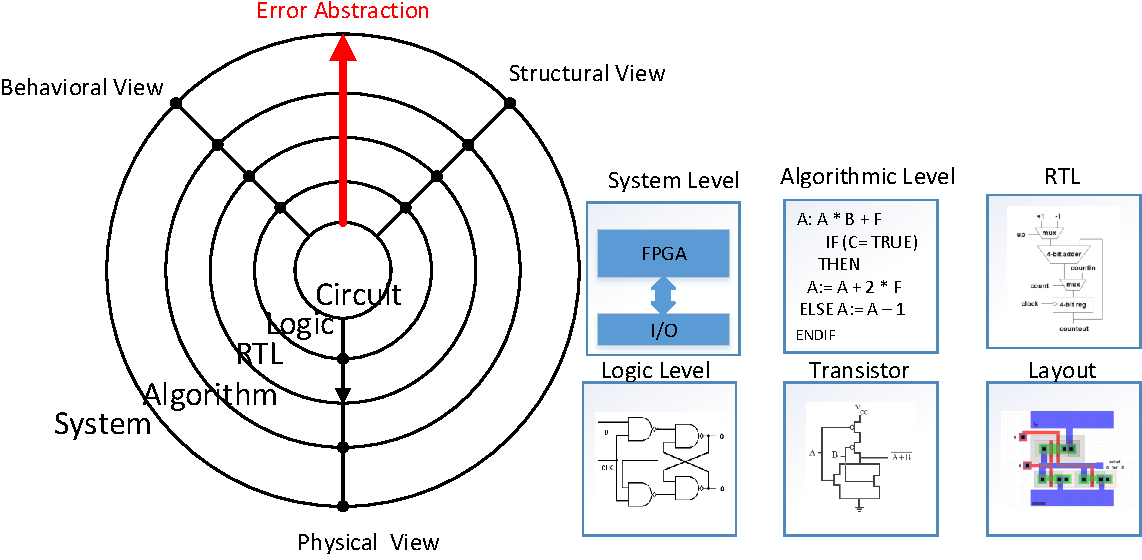
\includegraphics[scale=0.8]{Figures/ychart-block.pdf}
   \caption{Contribution of this work on Gajski-Kuhn chart.}
\label{fig:ychart}
\end{figure}



The objective of the thesis is to construct a high-level model from the faulty response observed at low-level circuit. This model provides the response of the system under fault. It can be described with Y-chart as shown in Figure~\ref{fig:ychart}, in which the high-level analysis (Behavioral View) based on the faulty response at the circuit level. At high-abstraction level the detailed of the implemented design is hidden from the designer making it more algorithmic and model based problem. In this work, we propose a solution --- simulate the low-level faulty response to the high-level behavioral model. The solution is based on the Hidden Markov Model, that uses the concept of hidden states  (stuck-at-fault) and observed states (signature) to find not only the hidden states of the faulty system but also accurately model the observed states. 


\begin{itemize}

%\item In this work, we will construct a high-level fault model that model the signature of the sequential circuits (ITC'99 benchmark). The high-level behavioral model based on the signatures from the sequential circuits.

\item This work will focus on the soft-error susceptibility for sequential circuits which are different from the combinational circuits. The error in the sequential circuit can be propagated back to the inputs, or circuits outputs can be affected for several consecutive clock cycles making the design more vulnerable.  
\item Our model will have the capability can efficiently model the worst case signature and the input vector correlated with this signature, through probabilistic modeling (HMM) and have the ability to measure the maximum and average signature probabilities. We also try to establish a relationship between the FPGA bits emulation information to the faulty models.



\end{itemize}

%%% Local Variables:
%% mode: latex
%% TeX-master: "../Document"
%% End:





%%- Uncomment the literature review for a thesis by articles -%%
%\begin{literaturereview}

%\end{literaturereview}

%%- First demo chapter -%%
\chapter{Related Work and Prior Work}


This chapter is dedicated to the revision of some of the fundamental concepts and current research in different areas related to this project: radiation effects on SRAM-FPGAs, soft-error, hard-error. Fault-injection, SEUs, Signatures, benchmarks for radation testing, and behavioral fault modeling. All of these topics are equally relevant for the purpose of this research that, ideally, places itself as an attractive research project.


 Most of the work done so far for soft-error analysis and evaluation is either on employing simulation framework, using fault emulation system on hardware, i.e., emulate faults on  FPGAs, and based on the efforts to find the analytical expression that represent the faulty behavior of the system

\section{Radiation Environment}

A Single Event Effect (SEE) results from a single energetic particle. When the particle strikes a sensitive node in a semi-conductor device, the ionization by the particle might produce a current pulse inside the device, which might cause soft or hard errors in the configurtaion memory of the device. Results in data corruption, transient disturbance, high current conditions (non-destructive and destructive
effects). SEE can if not handled well cause unwanted functional interrupts or in worst case catastrophic failures. Commonly, SEEs include single event upset (SEU), single event latch-up (SEL), single event burn-out (SEB), and single event transient (SET) etc as mentioned in Table~\ref{SEE-Summary}. SEEs may happen to electronic devices in these environments which is prune to the radiations. For example,
\begin{itemize}


   \item  Space (caused by space radiation)
    \item Air-plane (caused by atmospheric neutron)
    \item Close to nuclear reactor (caused by reaction neutron)
    \item Everywhere (IF caused by natural decay radiation in the materials of devices)

\end{itemize}



\begin{table}
\caption{Single Event Effects Summary}
\centering
\label{SEE-Summary}
\scalebox{0.4}{

   \begin{tabular}{c|c|c}
         \toprule
    \hline
     
     Single Event Upset (SEU)                  & corruption of the information \\ & stored in a memory element            & Memories, latches in logic devices                                  \\ \hline
    
    Multiple Bit Upset (MBU)                  & several memory elements \\ & corrupted by a single strike                & Memories, latches in logic devices                                  \\ \hline
    Single Event Functional Interrupt (SEFI) & corruption of a data path      & Complex devices with built-in state       \\ \hline
    Single Hard Error (SHE)                   & unalterable change of state in\\ & a memory element                     & Memories, latches in logic devices                                 \\ \hline
    Single Event Transient (SET)              & Impulse response of certain\\ & amplitude and duration                  & Analog and Mixed Signal circuits                      \\ \hline
    Single Event Disturb (SED)                & Momentary corruption of the\\&information stored in a bit             & combinational logic, latches in logic devices                       \\ \hline
    Single Event Latchup (SEL)                & high-current conditions                                              & CMOS, BiCMOS devices                                                \\ \hline
    Single Event Snapback (SESB)              & high-current conditions                                              & N-channel MOSFET, SOI devices                                       \\ \hline
    Single Event Burnout (SEB)                & Destructive burnout due to\\ & high-current conditions                  & BJT Power MOSFET    \\ \hline
    Single Event Gate Rupture (SEGR)         & Rupture of gate dielectric due\\&to high electrical field\\ & conditions & Power MOSFETs \\ \hline
    
    \bottomrule
    
    \end{tabular}
    }
\end{table}



\subsection{Faults Caused by Cosmic Rays in Digital Circuits}
\subsection{Single Event Effects Mechanism}
\subsection{Neutrons Effects on FPGA}





FPGAs are complex reconfigurable devices that comprise a wide family of different resources. The basic structure of modern FPGAs includes interconnect resources, clock-management resources, configurable logic blocks (CLBs), input/output
blocks (IOBs), and embedded blocks such as digital signal processors (DSPs), general-purpose processors, high-speed IOBs, and memories. CLBs are used to perform simple
combinational and sequential logic. These blocks are typically formed of look-up tables
(LUTs), multiplexers, flip-flops, and carry logic. Programmable interconnect resources, such
as routing switches, allow interconnecting CLBs, IOBs and embedded blocks to implement multiple systems (Buell et al., 2007).
The logic and routing resources in an FPGA are controlled by the bits of a configuration memory, which may be based on either antifuse, flash, or SRAM technology. The
design flow of FPGA-based systems as shown in Figure~\ref{fig:fpga-struct} adapted from ~\cite{hauck2010reconfigurable} involves the creation of a bitstream to load into the
device.



\begin{figure}[tb!]
 \centering
  \captionsetup{justification=centering}    
   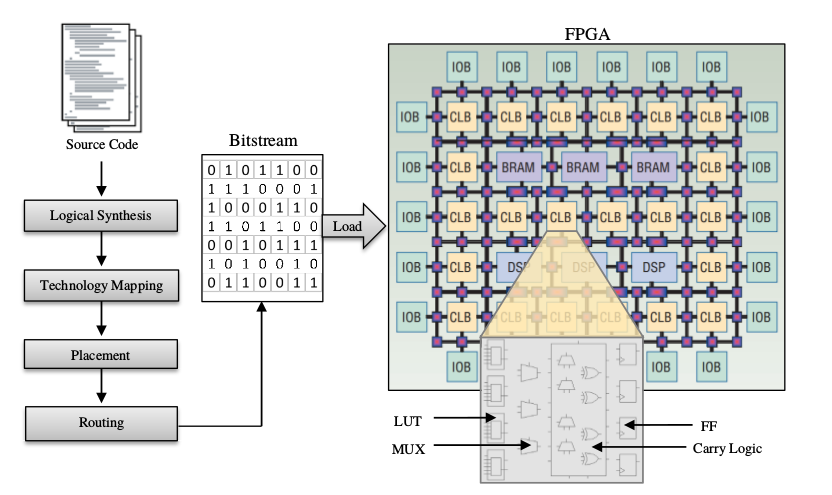
\includegraphics[scale=0.4]{figures/img/FPGA-structure.png}
   \caption{FPGA Structure and Design Flow}
\label{fig:fpga-struct}
\end{figure}



\subsection{Shielding Effect}

The process starts with the system design written
in a hardware description language (HDL), e.g., VHDL or Verilog. Next, the design is optimized and mapped into the FPGA’s available resources through logical synthesis,
technology mapping, placement, and routing. Finally, the generated bitstream downloaded into the device, and the device starts functioning according to the designer design.
Like any other semiconductor device, FPGAs are sensitive to radiation effects.
Mostly, these effects depend on the technology used to store the configuration data.
Regarding the impact of SEEs on reliability and functionality, FPGAs based on SRAM
technology are a particular class of devices. The foremost concern for SRAM-based FPGAs is
SEUs within the configuration memory. In such devices, this memory may represent more
than 80 percent of the total memory bits, increasing the probability of configuration faults.
Upset configuration bits may change the logic and routing of the implemented system, as
shown in Figure~\ref{fig:seu}, leading to functional failures in an unpredictable way. In contradiction, the primary concern for anti-fuse and flash-based FPGAs is SETs and SEUs within user flip-flops
and block memories. However, the configuration memory blocks of anti-fuse and flash-based
FPGAs offer a relative immunity to SEEs, but these devices have lower logic capacity and
cannot be reprogrammed an unlimited number of times, making SRAM-based FPGAs more
suitable for complex systems requiring frequent reconfiguration and adaptation~\cite{quinn2015validation, violante2004simulation}.

\begin{figure}
 \centering
  \captionsetup{justification=centering}    
   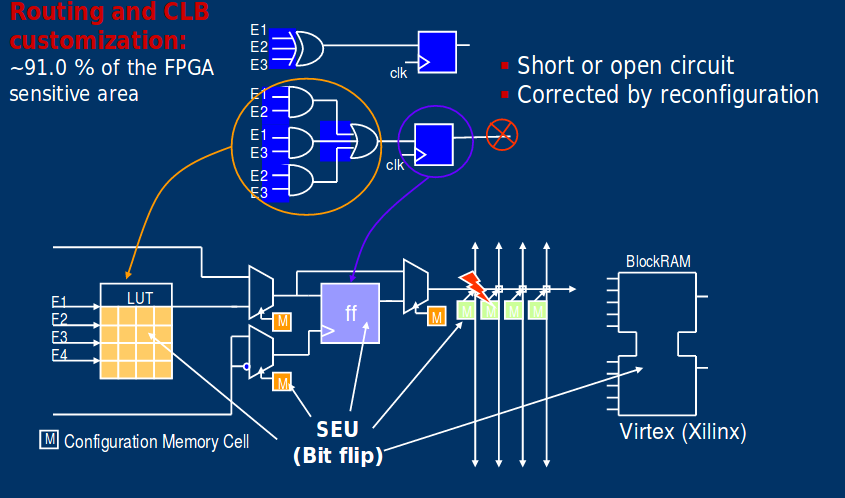
\includegraphics[scale=0.4]{figures/img/seu.png}
   \caption{Upset FPGA configuration bits may change the logic and routing.}
\label{fig:seu}
\end{figure}



%\subsection{Faults, and Failure}


\section{Design Verification by Fault Injection}



As we discussed before, SRAM-based FPGAs are particularly sensitive to SEUs. The configuration memory is the most sensitive part, by changing the configuration memory, may affect the overall functionality of the system. The work have done so far deal the SEU effects on FPGAs, combines the simulation, radiation, and emulation testing~\cite{quinn2015validation, violante2004simulation, hobeika2014multi, robache2013methodology, quinn2015using, souari2015optimization}. These papers described how they make the faulty behavior of the system to build an accurate representation of the system. The work presented in~\cite{quinn2015using} described the benchmark that can be used for the reliability and radiation effects study on FPGAs and microprocessors. FPGAs offer high densities and run-time programmability facility make inconvenient to use in the aerospace domain. But, FPGAs are sensitive to high-energy ions.  We need to study the sensitivity of SRAM-based FPGAs to heavy ions that show the suitability and analysis of effects of radiation on FPGAs when employed in space, e.g., usage of FPGAs in aircraft. The work presented in~\cite{hobeika2014multi} investigate the sensitivity of SRAM-based FPGAs devices not only for the simulation-based approach but also used emulation and radiation testing for evaluating the effects of SEUs. The work presented in~\cite{souari2015optimization} described the fault injection emulation in Xilinx FPGA based on the identification of critical configuration bits. Based on SRAM-based FPGAs, two aspects can be considered:

\begin{itemize}


\item SEUs may alter the contents of a register in the data path, or the content of the state register.
\item SEUS may alter the content of the configuration memory.

\end{itemize}



\subsection{Simulation}

The work presented in~\cite{robache2013methodology} discuss the fault simulation, fault emulation, and radiation testing. Starting from the simulation, I can interrogate how the authors used the concept of signatures to capture and reproduce the faulty behavior due to SEUs very early in the design process.
Radiation testing is an expensive approach and requires a state-of-the-art facility. The alternative to the radiation testing is the fault-injection approach.  The work presented in~\cite{hobeika2014multi} described the concept of faulty behavior signature. The work demonstrates how faulty behavior signatures allow building high-level models, e.g., high-level faulty model, i.e., Simulink, that reflects the faulty behavior of a combinational circuit represented at gate-level  (injected with one fault arbitrarily selected from a fault list). The main contribution of this work is to capture the effects of radiations on a circuit modeled at a low abstraction level and then abstract it to a  higher level. This challenge can be accomplished by introducing the concept of faulty behavior signature.  The fault injection tool that is used named - LIFTING.  The purpose of this tool is to study the effects of different types of faults on a circuit at gate-level. The tool used the stuck-at 0 and 1 are injected in each node of the design. The LIFTING is a simulation-based gate-level fault injection tool that used the circuit netlist file, e.g.  *.v file, input test vectors, and fault parameters as inputs produced two output files. The one is the golden report and the second consist of fault injection report. These two outputs are used to generate the signatures.  The signature represents the compressed faulty behavior of the circuit. The signatures consist of arrays of errors and their probabilities of occurrence. The signatures are either arithmetic or logic.  The third step is to make a high-level model that corresponds the low-level circuit. The work presented in this paper helps to make a faulty block with Simulink that reads a signature and generates errors according to the distribution.

\subsection{Emulation}
The emulation of SEUs in an FPGA is done by flipping the bit in the configuration memory. The emulation can be done by using the IP provided by the Xilinx named - LogiCORE. The work adopted the emulation work also proposed in the~\cite{hobeika2013flight}.  The work described a completed automated methodology to emulate SEUs on an FPGA efficiently. The authors used the reconfigurable flight control system based on a reference adaptive control model. The difference between the work presented in~\cite{hobeika2014multi} and~\cite{hobeika2013flight} is that; in~\cite{hobeika2013flight} the authors used the flight control system that is based on a linear plant model. Whereas, in~\cite{hobeika2014multi}the emulation is performed on the circuits (adder and multiplier). The work presented in~\cite{hobeika2014multi} used the SEU controller. The emulation is the four step process.

\begin{itemize}

\item Identification of an emulation zone.
\item Fault list generation.
\item SEU emulation.
\item Result Analysis.

\end{itemize}



The identification of an emulation zone used the concept of the essential bits which can be extracted by the Xilinx BitGen command. For example, 253227 bits are identified as the total essential bits in~\cite{hobeika2013flight}, among them, 57464 belongs to the interested essential bits. The step is used to minimize the time because an FPGA device contains millions of configurable bits, emulating a bit flip for every cell would be time-consuming. BitGen gives only the essential bits; that
considered critical bits. The second step generates the fault list. This action creates a list of the corresponding bit addresses (exact bit position to be emulated).  For example, authors observed 7000 emulation requests in~\cite{hobeika2013flight}.  The third step used auto-correct mode in which one bit is flipped at a time and the detect-only mode  (bit flips accumulation possible) where bits are flipped without correction. In the final step, an in-house script is used to characterize and quantify the design sensitivity to SEUs. This script is used to compare the results with the faulty one and fault-free. Authors observed 638 total number of failure in~\cite{hobeika2013flight}. Similarly, authors observed 80384 essential bits among them 2454 are considered as the interested ones for the adder circuit, for multiplier interested essential bits are 1314 among 92337 total essential bits.
The emulation can be performed on the Virtex 5. The 16-bit adder and  8-bit-by-8-bit multiplier are used as a testing circuit. The signatures are recorded in the accumulation mode. And, the estimation of the critical bits performed in the auto-correct mode.
The Emulation setup presented in~\cite{souari2015optimization} adopted the approach for the estimation by fault injection based on the sensitivity. Authors proposed the method in which fault are injected based on the specific bits configurations defined according to their contents and the type of FPGA resources. This new approach outperformed the traditional random fault injection with speed up factors to two orders of magnitude. This fault injection method based on the prioritizing specific subsets of configuration bits. These configuration bits are classified with the statistical analysis according to their values (0 or 1, and 2). The SEU controller a macro developed by Xilinx assuring fault injection, detection, and correction is used a fault injection engine in their experiments. The fault injection is prioritized using the following three steps:

\begin{itemize}

\item   {Classification of the configuration bits into subsets.
        a.  Bits set to 1/0 of LUT.
        b. Bits set to 1/0 configuring other than LUT.
        c. Bits set to 1/0 configuring other resources not identified as  potentially critical by bitgen.}
        
        
\item  {Estimating the number of critical bits of the set by randomly injecting faults in the bits of each set. This method helps to find the most critical zones of the FPGA.}

\item {Prioritized the fault injection in the identified (step-2) most critical zones.
These classification steps are done with the help of EBC and EBD files provided by the bitgen. The experimental results presented in [5] evaluated the SEU sensitiveness as well as bitgen efficiency. The results are evaluated between random fault injection with different prioritized bit subsets.  The first observation authors concluded - the bitgen did not accurately identify all the critical bits meaning the bitgen limitations. Second authors did the prioritizing the most sensitive subset. It would involve exhaustive fault injection. The authors used fault injection to get an estimated number of critical bits as well as the related estimation error. They used the term critical bit error estimate (CBEE). The authors claimed the CBEE observed for the random approach is higher than the observed under the bits subsets.  The ratio of observed critical bits (ROCB) observed for the random injection is far less than the different bits subsets.}



\end{itemize}



\subsection{Radiation testing}
The hardware setup consists of two Artix-7 board. Board A used as a reference and board- B is subjected to radiations. The board-A is not bombarded, and it hosted the counters, reference design error detection and signature computation, memories to store signatures and communication controller. A total 20 runs performed on the adder and 14 on the multipliers. Arithmetic errors for both approached DSP and LUT are observed (151 vs. 291 for DSP). This is due to DSP strategy; SEUs can add registers in the data path, leading to the sequential type of errors. The authors in this work compare the results from the fault simulation, fault emulation, and radiation testing. The purpose is to express as signatures, intended to reproduce the faulty behavior. They showed that simulation and emulation based signatures could contain the same error values as obtained with radiation but their probability of occurrence could significantly different. The arithmetic signature for TRIUMF to emulation is 85.3 % for adder and 84.8% for the multiplier. Similarly, the matching with the simulation of adder and multiplier with TRIUMF is 84.8 % and 100 % respectively.



%\subsection{Stuck-at Fault Model}
%\subsection{Functional Fault Model}
%\subsection{Open Fault}
%\subsection{Stuck-On and Stuck-Off}


\section{Fault Models}


\subsection{Stuck-at Fault Model}

\subsection{Functional Fault Model}






%\subsection{Benchmark for Radiation Testing}
The suitable selection of the benchmark for the radiation testing of microprocessor and FPGAs is a recently topic of ongoing research. The benchmarks are used to evaluate the performance under different architectures, technology, and compiler. There is no such standard benchmark employed to study microprocessor and FPGAs under the effects of radiations; make it difficult to assess the changes in fabrication technology, architecture, and circuitry. The work presented in~\cite{quinn2015using}described the software and hardware benchmark under the neutron test data. The unavailability of the such a benchmark for testing because radiation hardness assurance techniques are applied only to circuit layouts or manufacturing process. There is no standard test circuits available, researcher, used flip-flop or D-latches to compare their results. In recent years, radiation effects community shown interest to develop a standard set of circuits that include complex and realistic algorithms and can be adapted to different FPGAs.  Currently, without standard benchmark researcher used the following approach for testing:

\begin{itemize}


\item Homemade Design.
\item Circuits from Opencore.
\item Proprietary designs.
\end{itemize}


The problem with this approach as no two organizations used the same set of codes or circuits, difficult to make the comparison. There is a need for collaboration to make a suitable set of benchmark for reliability application and study the effects of radiation under the same conditions. The criteria used to set a standard benchmark including:

Repeatability of benchmark tests.
A representative of deployed computing workload.
Availability of fixed input vectors.
Cross-platform implementation.
The ability to repeat test itself is an important part of the standardized testing. By repeating the algorithms, the input test vector, the compilation, the synthesis setting help researchers to have the enough information. It is necessary to provide a wide variety of realistic algorithms so that the system can be tested as likely to the realistic application. Defining the input test vector is an essential step because many hardware errors can be observed under the specific set of the test vector. It is an open question which input test vector should be adopted, under the specific set of criteria. Finally, the implementation of the algorithms in portable languages help to use the same set of codes on the different platform. For example, assembly language for the microprocessors limit the ability to compare and port codes on the different platform. But the hardware benchmark developed in VHDL can ease the problem; the same circuit can be ported to any FPGA.

\textbf{FPGA Radiation Benchmark}

The FPGA benchmark mentioned in this paper is ITC'99 which is well defined ATPG benchmark. This benchmark meets all the requirements, e.g., realistic algorithms, input vectors, scalability, and portability. The circuits are implemented in the HDL so that it can be ported to different FPGAs. The first 15 circuits from the ITC'99 are adopted for the benchmark as shown in Table I.

\textbf{Software Radiation Benchmark}

The software radiation benchmark is harder to design than the FPGA radiation benchmark. The development of the standard set of algorithm that can be ported on different architectures would be a challenging task e.g., porting an algorithm to 16-bit microcontroller to GPU. The authors are interested in the software benchmark where the computational load can be divided into the parallel processes or run on a single core. The commonly used software benchmark comprises of fast fourier transform, matrix multiplication and quick-sort algorithm as they are commonly used in many applications and useful for the evaluating the reliability of parallel processors. The software benchmark comprises the following code.

\begin{itemize}
\item AES-128;
\item Cache test;
\item FFT;
\item Hotspot;
\item HPCCG;
\item Matrix Multiply;
\item Quicksort
\end{itemize}





\textbf{Radiation Testing}
The radiation testing is completed at Los Almos Neutron Science Center (LANSCE). The results are provided for the microcontroller, ARM cores, GPUs, and FPGAs. The B13 from ITC99 is used under the hardware benchmark suite; Virtex- 5 is used as a hardware platform. They also provide the result for the mitigation. For mitigation, they used X-TMR and VERI-Place. The failure in time (FIT) are decreased under mitigation, but the overhead is increased (circuit area increased).

\textbf{Hardware Benchmark Testing}
For the hardware radiation testing the authors used the B13 from the ITC’99 benchmark suite. The circuit is too small so it can be replicated 30 times, the implementation is done on the Virtex-5. Both unmitigated and mitigated version are tested. The results for FPGA radiation reports SDCs from the mitigated circuits normalized to the SDCs from the unmitigated circuits. Mitigated circuits are likely to fail at three times the rate of the unmitigated circuit, because of the increased size of the circuit from the mitigation process. The mitigated circuit cross-section is three times larger than an unmitigated circuit when SEUs accumulate. The authors conclude; the VERI-place mitigated circuits perform better than the X-TMR mitigated circuits.

\textbf{Software Benchmark Testing}
Software benchmark radiation testing is done on the flash-based microcontroller,  a ferroelectric-memory-based microcontroller, two ARMs, and GPUs. These components are tested with both mitigated and unmitigated codes. The results reported in the paper for two different microcontroller and two ARMs cores. For microprocessors: these microprocessors have very small SRAM the FITs are very small. In some cases, there is no error from the code during many days of testing. They also implemented the matrix multiplication, FFT, and Hotspot on NVIDIA K20 GPU and applied mitigation methods (ECC, ABFT, and DWC).  The purpose is to see the effect of overhead by applying the mitigation technique; the overhead has been increased as compared it with the unhardened configuration.
In short, the work presented in [3] evaluate a common set of hardware and software benchmarks to evaluate reliability and radiation effects on FPGA and microprocessors.





%\section{Fault-detection, mitigation and correction in the FPGA }


The impact of SEUs on SRAM FPGA devices has been studied in~\cite{bellato2004evaluating}. Many  techniques  have  been  proposed to provide highly reliable FPGA devices, e.g. radiation-hardened FPGAs~\cite{rockett2007radiation}, in-order to lower the effect of radiation-induced SEUs. However, radiation-hardened  SRAM  FPGAs  typically have  a  low  density, and  they  only  may  lower  the  probability of SEUs to occur but  not  completely avoid  them. Therefore, non radiation-hardened FPGAs, like the  Xilinx Kintex-7, are evaluated under a harsh radiation  environment~\cite{wirthlin2014soft}. Even on radiation-hardened FPGAs, the SEU rate in a low-earth orbit flight experiment can be up to 16 events per day~\cite{quinn2012orbit}. A wide  variety  of  SEU  fault  mitigation  techniques  for SRAM-based  FPGAs  have  been  proposed  during  the  past years. These techniques can be categorized into module redundancy techniques such as triple modular redundancy (TMR)~\cite{lyons1962use} and techniques that use scrubbing of the FPGA configuration memory~\cite{heiner2009fpga}. Also the combination of  both techniques has been shown to be able to increase the reliability of FPGA modules significantly ~\cite{ostler2009sram}. FPGA-based TMR approaches replicate a given module which shall be protected either statically or dynamically~\cite{angermeier2011runtime}. The different granularities of voted replicas  are evaluated in~\cite{bolchini2007tmr}. However, no upset rates and consequential no reliability figures are provided. Nevertheless, TMR techniques are  known to often cause an excessive and unacceptable overhead in terms of power  consumption and area. Since the intensity of a cosmic rays is not constant but may vary over several magnitudes depending on the solar activity, a worst-case radiation protection is far too expensive in most cases. A self-adaptive system is proposed in~\cite{glein2014self}, which monitors the current SEU rate and exploits the opportunity of partial reconfiguration of FPGAs to implement redundancy such as TMR on demand. 

Memory scrubbing is a well-known correction technique for the configuration memory of SRAM-based FPGAs. It consists on re-writing the configuration memory after the FPGA is configured to restore its original content. It is often a transparent operation for the running application. This is possible because modern FPGAs offer a dynamic partial reconfiguration (DPR) feature. The circuit that enables the scrubbing is commonly named scrubber. Additionally, readback is the process of reading the configuration memory of the FPGA after it is configured. Both processes (readback and scrubbing) can be used to implement different scrubbing methodologies as shown in~\cite{herrera2013design}. Scrubbing can be implemented using an internal or external interface as shown in~\cite{berg2008effectiveness}. When external interface is used, the scrubbing logic is implemented outside the FPGA. In the case of Xilinx FPGAs several external interfaces are available; however, the Select MAP interface has the highest data throughput. On the other hand, there is only one internal interface named ICAP~\cite{xilinx}. This internal interface can be accessed from the reconfigurable logic of the FPGA and it is a replica of the Select MAP interface. Also scrubbers can be implemented in software or hardware. The scrubbing process can be implemented using a microprocessor with the advantage of a high flexibility to implement different complex scrubbing methodologies but with lower configuration speeds and lower energy efficiency.

\section{Faults Behavioral Modeling}

%\subsection{Built-In Self-Test (BIST)}
%\subsection{All Test Pattern Generator (ATPG)}
%\subsection{Scan Chain Testing}


Intensive research has been done in the analysis of the faults for combinational circuits~\cite{mitra2005robust},~\cite{miskov2006mars} and sequential circuits~\cite{asadi2005soft},~\cite{miskov2007soft}. The most of the research work has been done is related to the transient fault analysis, soft error rate (SER) analysis and prediction, failure-in-time calculations. 

I summarize all those which related to this project at some extent as follows.

In~\cite{chen2017fault} this paper proposes the fault propagation process between the different subsystem of the
main system, combined with the finite state machine, but they did not provide any experimental data to support their idea. Only, MTBF is provided.

In~\cite{li2016monte} in this paper, Monte Carlo technique is used for the soft error analysis of the sequential
circuits. They perform the logic simulation for latch-level error propagation to estimate the SEUs. This work is mainly focused on the convergence of the variance of the estimate of SEUs.
They insert the fault into the simulator and observe it to the output. Apply the Monte Carol technique
to find the number of samples and the time for the estimation of the error
  
  
In~\cite{kapare2016automated} in this work, they propose a methodology to estimate the output quality of approximate
sequential circuits (faulty circuits) based on finding the analytical expressions for predicting
approximation errors from statistical data gathered from performing limited characterization of the
approximate circuits (faulty circuits). They propose a methodology for estimating/predicting the output
quality of a faulty circuit. They want to accurately predict the error behavior. Simulation-based results. Fault assumptions. Drive the analytical expression for the faulty
circuits. Compare the results of the analytical expression and the simulation to observe the error
difference. They did Curve fitting for analytical expression. 

In~\cite{ebrahimi2015comprehensive}  the key idea behind this paper to present the result for SER analysis on an embedded
processor. There platform employs a combination of models at device level, gate level error
propagation and at architectural level.
Limitation: The main limitation of this work - as they claimed they performed all the experiment on
the embedded processor but in experiment section instead using a processor chip, they used the
processor core and drive all the results via simulation of this core under the assumption of the fault. While using processor core under the radiations the primarily concerns is for the cache memory instead
of the core itself.

In~\cite{ubar2014modeling} this work is based on the Simulation, transformed the circuit into their required tool format, then they
insert the fault on different nodes and calculate the SER. The main limitation of this work is the tools limitation for the transformation of the circuit.



In~\cite{mirzadeh2014modeling} In this work, author proposed a fault behaviour model developed with a neural network
concept in a novel way. The neural networks (NNs) structure was used to synthesize the faulty output of a
circuit at a high-level of abstraction. All the strategies that were proposed in this research have novelty;
and effort is exercised to find an appropriate structure for the neural network. The idea is good to make a model with NNs. But it underestimate the power of NNs for
smaller circuits



In~\cite{ranjan2014aslan} this technique is used to estimate the output quality of a faulty circuit which uses the concept
of unrolling the circuit each clock cycle and compares this faulty unrolled circuit with the original circuit
using a quality evaluation circuit and generates some vectors, which indicate the quality of the circuit
at that cycle. Unless the quality constraints are satisfied. The faulty circuit is unrolled every cycle with incremental improvements in each cycle. Thus,
if the desired output quality is high, the cost of unrolling and analyzing error metric also increases
substantially.

In~\cite{brkic2014symbolic} the key idea behind this paper presents a symbolic analysis method for unreliable logic
gates. The limitation of this paper is that they consider only the example of two input NAND gate
and their test platform and drive the mathematical fault model. This is too small circuit for symbolic
algorithm validation. They also assumed the fault in the design.

In~\cite{chan2013statistical} this paper addresses the estimating output quality of a faulty hardware circuit by pre-
characterizing the relationship between Error metric behavior and characteristics of approximate
hardware circuits. These values are stored in lookup tables which are used to retrieve Error metric
composition for a given approximate hardware module and then compose error metrics for output
quality using regression-based models. This approach also takes into consideration the input
distributions of the faulty circuit. There are certain disadvantages of using this technique. First, this technique is limited to
only adders and circuits constructed using blocks of adders. It is not scalable to multipliers or sequential
circuits as the regression-based model is not applicable for these circuits as this approach requires
error metrics to be additive in some way to use regression-based approach. Secondly, the
characterization time increases as the number of nodes increase in the circuit as the larger number of
simulations are required. In addition, the memory overhead required is large as we need to store
multiple lookup tables for this approach. Hence, this technique is not particularly useful for complex
circuits or for circuits having a high number of nodes.





In~\cite{shazli2011high}, in this work, the Soft Error Rate (SER) computation problem is modeled as a Boolean
Satisfiability (SAT) problem and SAT solvers are used to compute SER for combinational and
sequential circuits. They used an automated flow to convert combinational and sequential behavioral
descriptions into equivalent SAT instances. The use of Boolean Satisfiability (SAT) approaches, to
model soft errors in early design stages presented. The transformation of the circuit into Boolean Satisfiability SAT problem is challenging task
itself, plus its too hard for complex circuits. Only Simulation work is presented.



In~\cite{al2010fault}, the objective of that work was to investigate the design of soft error tolerant sequential
circuits based on adding redundant states at the state diagram level. The objective of adding redundant
states is to guarantee tolerance of all single soft errors of states with high probability of occurrence.
They also propose technique to get the minimum number of redundant states that will add minimize
hardware overhead. They implement a tool for computing soft error reliability for sequential circuits based on
the Monte Carlo simulation. They develop an algorithm that add redundant states that create an area
overhead problem. Monte-Carlo estimation method to estimate the failure rate by injection faults
during simulation. All the work based on the simulation. Convert the circuit into respective FSM, inject
faults randomly, simulate it and propose the redundant states.




In~\cite{yu2010scalable}, this paper, authors developed novel and efficient ways to sample logic circuit behavior,
model the impact of soft errors, and estimate the circuit reliability. Their method was described that
used the probabilistic transfer matrices to calculate signal and error probability distributions in the
sequential circuits at the logic level. This work is mainly focused on finding the signal probabilities at the gate level. To do so
they partition the combinational part of the sequential circuit, and then find the probabilities of each
individual gates.

In~\cite{lingasubramanian2010probabilistic}, this work, they calculated the maximum error in digital logic circuits and the respective
worst-case input pattern, through maximum a posteriori hypothesis, using a Shenoy-Shafer algorithm.
They showed the importance of handling maximum error behavior for achieving fault tolerant
computing machines. They studied the circuit-specific error bounds for fault-tolerant computing. This work is mainly focused on finding the signal probabilities; convert the signal
probabilities into angles. Use conditional error model, which is not the case in real-time testing.
Simulation and assumption work. They calculated the average output error in sequential circuits and
studied the transient error behavior across different time instances, using a dynamic time evolving
probabilistic error model.

In~\cite{miskov2008modeling}, Markov chain for the steady-state behavior of the sequential circuits, Symbolic framework
based on the BDD/ADD is presented. They did the Single Error Rate (SER) evaluation, purposed to do
for the gate sizing, find the gate size that has the highest soft error impact based on this recommend
different gate size for the transistor technology. They use the only Simulation, assume fault occurs, suppose the glitch size, and assign the
probabilities in the HSPICE simulator. They make the model of the faulty circuit by supposing it gets
fault make a model with Markov chain, ADD/BDD and then compare it with the simulation using the
HSPICE. They also assume that an error occurs only in the first clock cycle of a w-cycle simulation with
no new errors occurring in subsequent cycles. It has difficulty simulating circuits over many cycles
because of the way it employs the time-frame technique. The circuit size and the number of primary
inputs and outputs grow linearly with the number of simulated cycles, and memory usage becomes
unmanageable after a few simulated cycles. Another source of inaccuracy in their work is that it
assumes an error occurs only in the first clock cycle of a w-cycle simulation, and no new errors arrive in
subsequent cycles.

In~\cite{miskov2007mars}, the symbolic framework based on Binary Decision Diagram (BDD) / Algebraic Decision
Diagram (ADD) to analysis sequential reliability is presented in this paper. They calculate how much the
gate output is suspected of an error. The MES is calculated at the electrical (transistor) level regarding
the duty cycle, signal amplitude (voltage), and the gate error probability of individual gates associated
with different input probabilities. They use only Simulation, assume fault occur, suppose the glitch size, Simulate by inserting
glitch of different time-period. Find the gate error probability of individual gates. 


In~\cite{miskov2007mars}, n this work, they estimate the likelihood that a SET in a sequential circuit will lead to errors
in clock cycles following the particle hit, and find after the hit (which is an assumption) how many clock
cycles needs to get the SER below the threshold level. The main idea was to allow for symbolic modelingand efficient estimation of the susceptibility of a sequential circuit to soft errors. A symbolic modeling
methodology for efficient estimation of the soft error susceptibility of a sequential circuit.
Limitation: They solved the problem with the analytical approach. Almost similar to the previous work.~\cite{miskov2007mars},~\cite{miskov2008modeling}. There main concern after particle hit (in experiment they did not performed this) how many
clock cycles will it take to get SER decrease.


In~\cite{das2007monitoring}, Error Monitoring scheme to detect the Transient Error. The idea presented in this work has a worth to compute the error for each stage
independently. But they didn't provide they experimental setup details, no details for the how the fault
occurs in their system.

In~\cite{asadi2005soft}, they provide the multicycle analytical framework to analyze the multi-cycle error
propagation. The major limitation to their work is the measuring unit the used in their work “mean time
to manifest error.” The common terminology for this kind of work is SER. This is the simulation work,
with the assumption that the fault will occur in the flip-flop and proceed to other flip-flop. They did not
consider the fault occurs in the combinational logic of the sequential circuit.

In~\cite{miskov2010multiple}, the key idea presented in this paper is to analysis the susceptibility of the circuits outputs
errors originating from the single or multiple fault transients faults. They are keener to find the part of
the circuit that has the highest error generating probability.
The Simulation work, they assumed the fault scenarios for their benchmark. Focus only on the
SET. They droved the errors for flip-flop and gates separately





In~\cite{svenningsson2010model}, In this paper the idea presented how model-implemented fault injection can be utilized to
simulate the effect of hardware related faults in embedded systems. Model level and hardware level
fault behavior comparison is presented.
The limitation of this work; simulation work, they assume the fault scenarios for their pedal examples. Although, the
perform the emulation on the microcontroller as well but they develop a separate tool which change
the bit value in the register or memory cell of the assembly language.


In~\cite{hayne1999behavioral}, in this work, they proposed two tools, which facilitate the fault simulation of behavioral
models, described using VHDL. The tool is the Behavioral Fault Mapper (BFM). The BFM algorithm
accepts a fault-free VHDL model of the design (combinational circuit) and a fault list of N faults from
which it produces N faulty models. The assumed 8 different fault models e.g., Stuck-Then, Stuck-Else,
Assignment Control, Dead Process, Dead Clause, Micro-operation, Local Stuck-data, Global Stuck-data. The faulty models they constructed in their work from the faults based on the assumptions
and deliberately make them fail. There is no emulation performed.

In~\cite{hachtel1996markovian}, Modeling the Probabilistic Behaviour of the Finite State Machine, calculating the steady state
behaviour of the circuit and used for estimating the switching activity of the circuit for the purpose of
power evaluation. They showed how steady-state probabilities of very large FSM’s can be computed by
symbolic ADD-based algorithms. The limitation of this work is to convert the design FSM into ADD, many assumptions, and simulations only.









\label{related}
\section{Relation to State-of-the-Art}
The work done so far [1, 2, 3, 4, and 5] evaluated and quantified the SEU effects by performing simulation, emulation, and radiation on an SRAM-based FPGA. Implemented a design, observed its faulty behavior in the presence of SEU and extracted the corresponding fault model. Presented an automated methodology to efficiently used the SEU controller. Discussed the fault injection on the specific subsets rather than random and discussed the selection of the suitable benchmark for FPGA and microprocessor radiations. 




%%% Local Variables:
%%% mode: latex
%%% TeX-master: "../Document"
%%% End:


\chapter{Proposed Approach}

This chapter is dedicated to the methodology that we propose to exert to achieve the objectives of this research project, i.e. Methodology and Algorithms for High-level Modeling of Cosmic Radiations Impacts on Electrical Systems.





\section{Relation to State-of-the-Art}
Starting from the background, the facts established in the Chapter~\ref{intro}--- the digital circuits vulnerable to radiations require high-reliability requirements. The faults due to particle strikes cause different effects in the system behavior, e.g., stuck-at-fault. As discussed in~\ref{related}. In the digital sequential circuit, a single event upset cause a multiple faulty response of the underlying circuit. Consider this faulty response occur due to a node in the circuit at stuck-at-fault, e.g., 3-bit counter as shown in Figure~\ref{fig:counter} stuck-at-1$\rightarrow O_0$. This stuck node response can propagate to multiple outputs, as shown in Table~\ref{s@1-O0} and produce multiple erroneous outputs. The way this SEU interrupt at high-level of abstraction could typical manifest multiple correlated; "change in states of the design", and "change in signature values." Inorder to model the fault occur at low level, and make the model of the faulty response of the circuit at high level of abstraction, I propose to use the Hidden Markov Model. 



\begin{figure}[tb!]

 \centering
  \captionsetup{justification=centering}    
   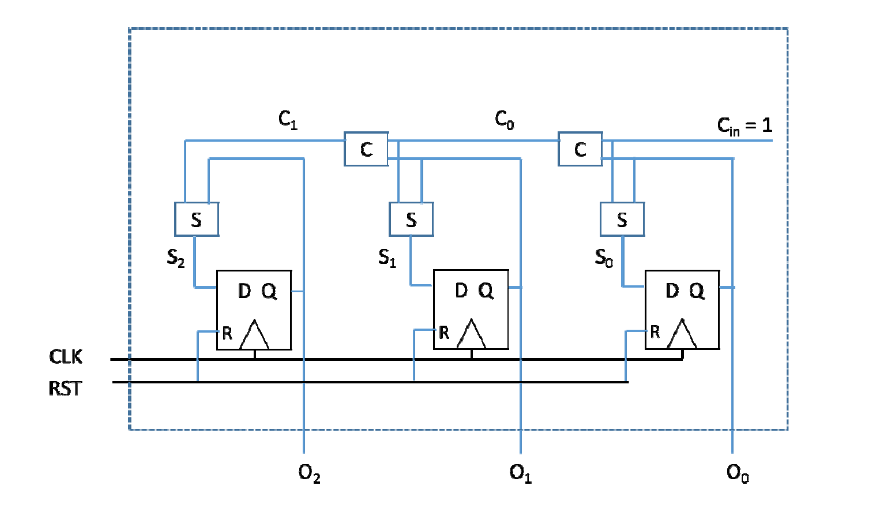
\includegraphics[scale=0.6]{Figures/counter.png}
   \caption{Signature Generation}
\label{fig:counter}
\end{figure}



\begin{table}[tb!]
\center
\caption{stuck-at-1$\rightarrow O_0$}

\label{s@1-O0}

\begin{tabular}{|c | c| c | c| } 
 \hline
 \rowcolor{lightgray}
Faulty Value (Binary) & Faulty Value & Original Value & Arithmetic Signature   \\ 
\hline

 
 
 001& 1 &0 & -1  \\
 \hline
 011 & 3 & 1 & -2 \\ 
 \hline
 
 101 & 5 & 2 & -3 \\
 \hline
 111& 7& 3& -4 \\
 \hline
 001 & 1  &  4& 3 \\
 \hline
 011 & 3 & 5 &2  \\
 \hline
 101 & 5 & 6 & 1 \\
 \hline
 111 & 7 & 7 & 0 \\
 \hline
 
 
\end{tabular}
\end{table}




\section{Why Hidden Markov Model?}


We used the HMM for modeling and analysis of sequential circuits susceptible to soft-errors. We prefer to use the HMM analysis over the other modeling techniques, e.g., BDD/ADD or Boolean Satisfiability problem (SAT), Monte-Carlo sampling, approximate approaches, symbolic methods for efficient estimation, simulator methods. As all these techniques require to transform the circuit into their respective tool or mathematical notation. While in HMM we can directly make the model just looking into the signature values. The faulty behavior of a sequential circuit can be analyzed by using the HMM.  

In order to make the HMM. We need to have two copies of the original circuit --- named Fault-Free circuit, and a Faulty circuit (\textit{hit circuit}). The Fault free circuit is used to collect the correct behavior of the circuit (fault-free outputs), and faulty is used to collect the faulty response of the circuit (faulty output). The difference between them give us the signature as shown in the Figure~\ref{fig:SG}


 \begin{figure}[tb!]

 \centering
  \captionsetup{justification=centering}    
   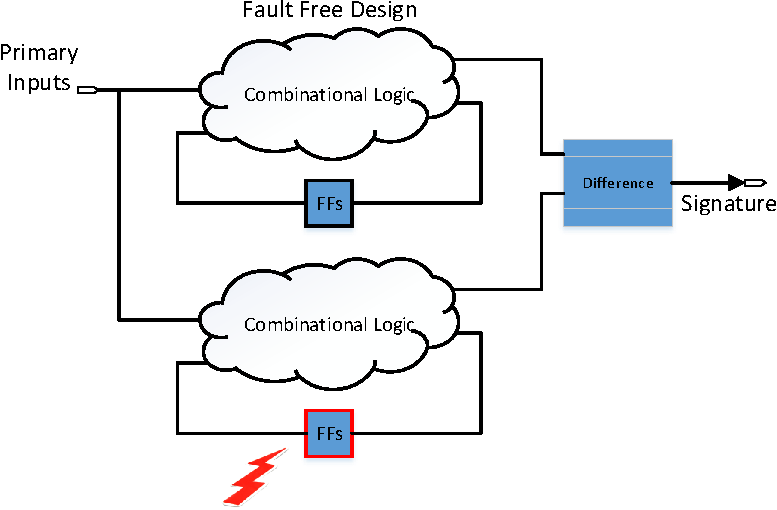
\includegraphics[scale=0.8]{Figures/signature1.pdf}
   \caption{Signature Generation}
\label{fig:SG}
\end{figure}

The HMM is based on  the two things:a) Observable States, and b) Hidden States. If we closely observe above mentioned example, we realized that in this scenario --  signatures are the observable state, and the fault occur due to the bit-flip that cause some node in the circuit to stuck, stuck-at-1 $\rightarrow$ $O_o$ is the hidden state. In this thesis, we propose a method based on the Hidden Markov Model to evaluate the severity of the faulty behavior induced by the SEUs as a high level behavioral level. 







\section{Modeling Hidden Markov Model}

The Figure~\ref{fig:HMM-air} shows the basic HMM applied to the FPGA based fault emulation system. The HMM is called hidden because only the outputs emitted by the system (FPGA under radiation/ Fault Emulation) are observable (signatures --- in ours problem domain), not underlying states of the system (Stuck-at-fault). The HMM can be visualized as a simple finite state machine. The HMM has a strong statistical foundation; it has the ability for efficient learning algorithm, which can take place directly from the raw sequence data. \textbf{The problem in hand:} can be solved by using the HMM as we can observe the sequence of signatures, but we do not know the which states (stuck-at-node) of the system went through to generate that particular signature. The analyses of Hidden Markov Model seek to recover the states from the observed data.

\begin{figure}[tb!]

 \centering
  \captionsetup{justification=centering}    
   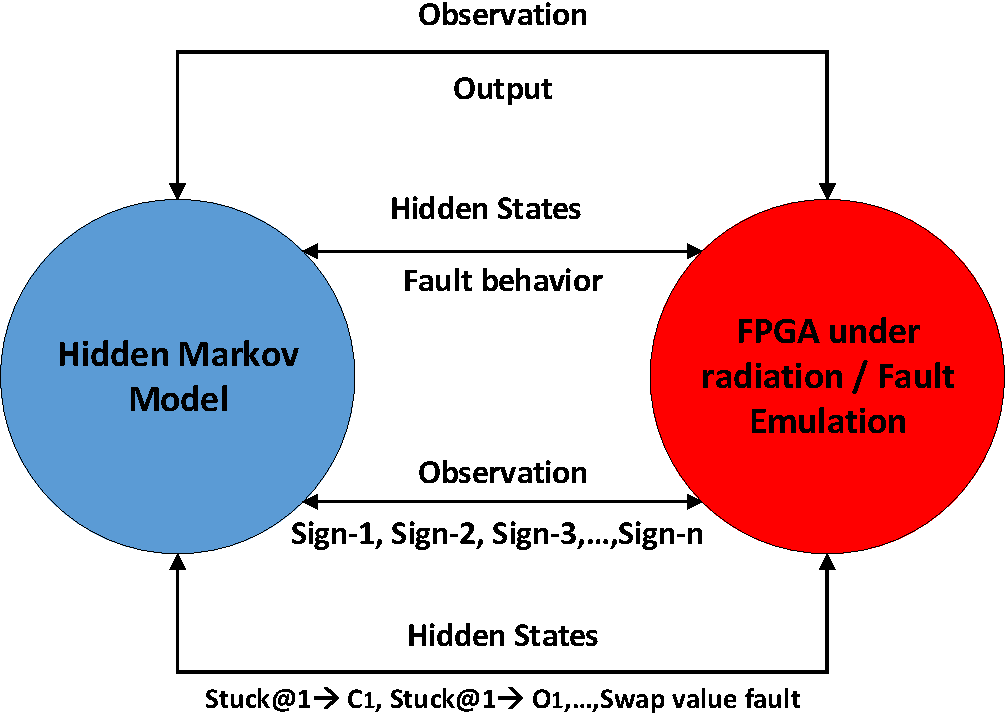
\includegraphics[scale=0.8]{Figures/HMM-air.pdf}
   \caption{Hidden Markov Model to the FPGA based fault emulation system}
\label{fig:HMM-air}
\end{figure}






Hidden Markov Model is a statistical model in which a system can be modeled is assumed to be a Markov process with unobserved, i.e., hidden states. A Markov process  is a stochastic process that satisfies the Markov property -- \underline{memorylessness}, meaning, a process that satisfies the Markov property if the prediction of the future of the system output based solely on its present state, it is independent of the future and past states. Inorder to apply the HMM, we need a system that generate probabilistic output patterns in time, e.g., faulty response of the 3-bit counter, as a result the node is stuck-at-fault. Afterwards, we need to look at the system and need to know which state of the system give that particular output ---  the underlying system is hidden. For example, in the case of a three bit counter, the observed sequence is the "signature" and the hidden is the "stuck-at-node." Now, we wish to devise a model to predict "stuck-at-node", without actually knowing about the node. It is important to note that the number of states in the hidden process and the number of observable states may be different. 


In the 3-bit counter example, there are total n-nodes where the signal can get stuck (stuck-at-1, and stuck-at-0) both are possible. and we can get the  different signatures (chapter Preliminaries derive signatures for all the nodes). Here for simplicity, I can give the example of four different signatures and construct the HMM. The signarures are: \textit{Sign-1, Sign-2, Sign-3, and Sign-4}. The observed signatures are probabilistically related to the hidden process. We can model such process using a hidden Markov model, where there is an underlying hidden Markov process changing over time, and a set of observable states which are related to somehow to the hidden states.


The figure~\ref{fig:HMM-3-bit} shows the Markov model for the hidden and the observable states for the 3-bit counter example. The hidden states are (stuck-at-nodes), and observable states are  the signatures. 


\begin{figure}[tb!]

 \centering
  \captionsetup{justification=centering}    
   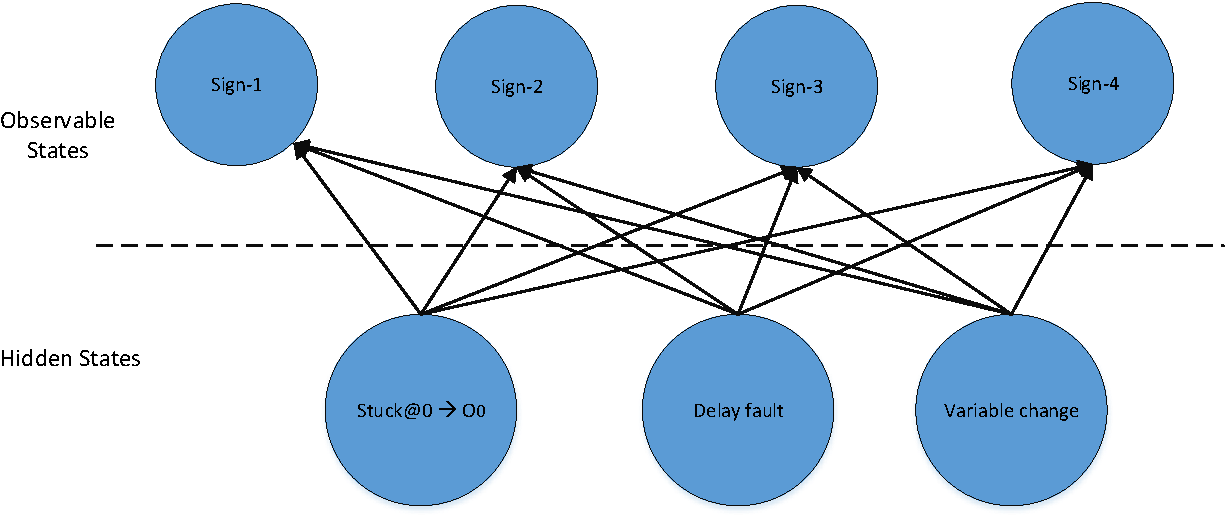
\includegraphics[scale=0.8]{Figures/HMM.pdf}
   \caption{HMM model 3-bit counter.}
\label{fig:HMM-3-bit}
\end{figure}

\subsection{Probabilities in a HMM}

There are three important things to know about the probabilities in HMM.

\begin{itemize}
\item The connections between the hidden states of the system, and the observable states of the system represent the probability of generating a particular observed state given that the Markov process is in a particular hidden state.

\item The probabilities entering into the observable states will sum to "1." 

\begin{center}
$Pr(Sign-1|Stuck) + Pr(Sign-1|Stuck) + Pr(Sign-1|Stuck)  = 1 $
\end{center}

\item In addition, probabilities define the Markov process, we have another matrix termed as "confusion matrix", which contains the probabilities of the observable states given a particular hidden state. The following matrix is the confusion matrix for the 3-bit counter example.


\begin{center}


CM = \bordermatrix{~& Sign-1 & Sign-2 & Sign-3 & Sign-3\cr
                  Stuck@1\rightarrow{C_0}& 0.60 & 0.20 & 0.15&0.05 \cr
                  Stuck@1\rightarrow{C_1} & 0.25 & 0.25 &0.25 &0.25\cr
                  Stuck@1\rightarrow{O_0} & 0.05 & 0.10 &0.35 &0.50\cr}
\end{center}
\end{itemize}


\subsection{HMM Parameters}

A hidden Markov Model is described as $(\Pi, A, B)$, Where,


\begin{center}

$\Pi = (\pi_i)$ initial state probabilities vector;

$A = (a_ij)$ state transistion matrix;  \hspace{0.3cm} $P_r(x_i | {x_j}_{t-1})$

$B = (b_ij)$ confusion matrix;     \hspace{0.3cm}        $P_r(y_i | x_j)$


\end{center}  

\textbf{Hidden States:} The true states of the system that may be described by a Markov Process, e.g., Stuck-at-1, some particular node.

\textbf{Observable State:} The state of the process, visible, e.g., Signature (difference between original output and faulty output).

\textbf{$\Pi Vector$:} contains the probability of the hidden model being in a particular hidden state at time t = 1.

\textbf{state transition matrix:}  holding the probability of a hidden state given the previous hidden state.

\textbf{confusion matrix:} containing the probability of observing a particular observable state given that the hidden model is in a particular hidden state. 



Once a system can be modeled as a HMM, it helps to find three problems. We model them according to our problem, i.e.,

\begin{tcolorbox}[width=\textwidth,colback={gray},title={Evaluation },colbacktitle=gray,coltitle=black]  

Find the probability of an observed signature given a HMM.  
\end{tcolorbox}


\begin{tcolorbox}[width=\textwidth,colback={gray},title={Decoding },colbacktitle=gray,coltitle=black]  

Finding the hidden states (stuck-at-fault) that most probably generated an observed sequence. 
\end{tcolorbox}

\begin{tcolorbox}[width=\textwidth,colback={gray},title={Learning },colbacktitle=gray,coltitle=black]  

The third problem is generating an optimized HMM given a sequence of signatures (observations).
\end{tcolorbox}



\section{HMM Application for Signature}

Hidden Markov Model can give the answer of three major questions, compute the probability of a given sequence of signatures, compute the most probable sequence of states, given a sequence of observations and learn the best model, given an observation.

In order to find the solution of these three questions:


\textbf{The Three basic HMM Applications}

\begin{itemize}
\item Problem 1 : Probability Evaluation
 \begin{itemize}
 \item How do we efficiently compute the $P(O|\Pi)$ from the given observation sequence $O = {O_1, O_2,...,O_n}$.
 
  \begin{itemize}
  \item The possible solution is given by the Forward and Backward procedures.
  \end{itemize}
 \end{itemize}
\end{itemize}

\begin{itemize}
\item Problem 2 : Optimal State Sequence
 \begin{itemize}
 \item Given observation sequence $O = {O_1, O_2,....,}O_n$ and model $\Pi$ how do we choose a hidden state sequence $Q={q_1,q_2,q_3,...q_n}$
that is optimal, i.e., best explains the data. 
  \begin{itemize}
  \item The solution is provided by the Viterbi algorithm.
  \end{itemize}
 \end{itemize}
\end{itemize}



\begin{itemize}
\item Problem 3 : How do we adjust the paramters of the model $\Pi = {\pi, A, B}$ to maximize the likelihood $P(O|\pi)$ 
 \begin{itemize}
 \item Given observation sequence $O = {O_1, O_2,....,}O_n$ and model $\Pi$ how do we choose a hidden state sequence $Q={q_1,q_2,q_3,...q_n}$
that is optimal, i.e., best explains the data. 
  \begin{itemize}
  \item The solution is either Expectation-Maximization or Baum-Welch re-estimation.
  \end{itemize}
 \end{itemize}
\end{itemize}









\subsection{Evaluation Application}

For probability evaluation we need to compute the likelihood of an observation sequence $O = {O_1, O_2,...,o_t}$ given a particular HMM model $ \Pi = {A, B, \pi}$. The computation of this probability involves all the possible hidden state sequence and evaluate the corresponding probability. 

\begin{itemize}

\item  $P(O | \Pi) = \sum\limits_{\forall Q}^{} P (O | X, \Pi) P (X, \pi)$ 

\item For a specific state sequence $X = {x_1, x_2,...,x_t}, P(O | Q, \Pi):$

 \hspace {0.2cm} $P (O | X, \Pi) = \prod_{t=1}^{T} P (o_t | q_t, \Pi) = \prod_{t=1^{T} b_{x_t} (o_t)}$
 
 \item The probability of the state sequence $X$:
 \\
 \hspace {0.2cm} $ P (X | \Pi ) = \pi_{x_1} a_{x_1 x_2} a_{x_2 x_3},...,a_{x_{T-1} x_T}$
 
 \item The final expression we get:
 


$P (O | \Pi ) = \sum\limits_{x_1, x_2,..., x_T} \pi_{x_1} b_{x_1} (o_{x_1}) a_{x_1 x_2} b_{q_2} (o_{x_2}),..., a_{x_{T-1} x_T} b_{xT} (o_{xT})$

\item If there are $N^T$ possible state sequence, this approach becomes infeasible to apply or implement even for the smaller circuits.

\begin{itemize}
\item For N = 5 and T = 100, the order of magnitude --- $10^7$
\end{itemize}
 

\end{itemize}

This problem can be solved by using the Forward Algorithm:

\textbf{Example:} Consider an example where we have a number of HMM (a set of trplet $(\pi, A, B)$) describing different systems, and a sequence of observation, e.g., you will get these system by performing radiation/fault emulation experiments for hours and hours of testing. You have number of HMM in simulink library and want to know which HMM most probably generated the given sequence (signature).


We will use the forward algorithm to calculate the probability of an observation sequence given a particular hidden Markov Model, and find the most probable HMM. Suppose that you have a HMM that describe the stuck-at-node, and we also have a sequence of signatures. Suppose the stuck-at-nodes works in this order $(stuck-at-c_0)$, $(stuck-at-c_1)$, $(stuck-at-O_1)$, the signatures: Sign-1, Sign-2, Sign-3. There is some hidden relationship between stuck-at-node and the signatures, we can make a "Trellis" diagram as shown in Figure....


From trellis figure we conclude the following:

\begin{itemize}

\item Each column in the trellis represents the possible state of the stuck-at-node and each state in column is connected to the each state in the adjacent column.

\item The transition between the states --- state transitions has the probability provided by the "state transistion matrix."

\item Each column in the signature observations at that time: the probability of this signature observation given anyone of the above stuck-at-node state is provided by the confusion matrix. 

\item As mentioned above one of the possibility of calculating the probabilities of the observed states would be find each possible sequence of the hidden stuck-at-node states and sum all these probabilities. Just for this example, there would be $3^3 = 27$ possible sequences, its extremely complex to do this. So, we used the forward algorithm that can calculate the probabilities of observing a sequence recursively given a HMM.

\end{itemize}

\textbf{Forward algorithm Steps:}

We need to calculate the probability of observing a signature recursively given a HMM. 

\begin{enumerate}

\item The first step is the initialization step at t = 1 when there is no path to the state. The probability of being at state at t = 1 is actually the initial probability:
\begin{itemize}


 \item $P (state | t = 1) = \pi $
\item The initial probability at t = 1 is the probability multiplied by the associated observation probability.
$\alpha(j) = \pi(j) b_i (O_1)$
\end{itemize}

\item Second, we need to define a \textbf{partial probability} which is the probability of reaching an intermediate state in the trellis.

\begin{itemize}

\item For example, the T-long signature sequence: $(Y_k1, Y_k2,..., Y_kT)$, the partial probabilities $\alpha 's$. Figure shows the Trellis diagram. Calculate the probability of reaching an intermediate state in the trellis diagram as the sum of all possible paths to that state.

\item The partial probability of state $j$ at time $t$ is $t(j)$, to calculate the partial probability:

$\alpha_t(j) = P (observation | hidden state is j) \times P (all paths to state j at time t)$

\item The partial probabilities for the final observation hold the probability of reaching those states going through all the possible paths. The sum of these final partial probabilities is the sum of all possible paths. 

\hspace {4.5 cm}$\alpha_{t+1}(j) = b_jk_{t+1} \sum\limits^{n}_{i = 1} \alpha_t(i) a_{ij}$




\end{itemize}
\item This expression can be used to calculate the $\alpha$. We can find the probability of an observation given HMM. The probability of the sequence given the HMM is then the sum of the partial probabilities at time t = T. This is called termination step.
 
 \hspace {4.5 cm}$P(Y^K) = \sum\limits^{n}_{j=1} \alpha_T (j)$

\end{enumerate}







\subsection{Decoding Application}







To design it for the decoding application there are two possibilities to use either viterbi decoding algorithm or posterior decoding. The viterbi gives the most likely sequence while posterior decoding gives the most likely state at each position. Here, we are more focused on the sequence of hidden states that give the respective signatures, in this case viterbi algorithm is preferable. The decoding capability of HMM helps to find the sequence of the stuck-at-fault that generated the given signatures. In the FPGA fault emulation and radiation experiment we are interested to find the stuck-at-fault nodes of the system as they represent some valuable information that can later be used to give to the Simulink model as shown in Figure~\ref{fig:HMMsig}.



\begin{figure}[tb!]

 \centering
  \captionsetup{justification=centering}    
   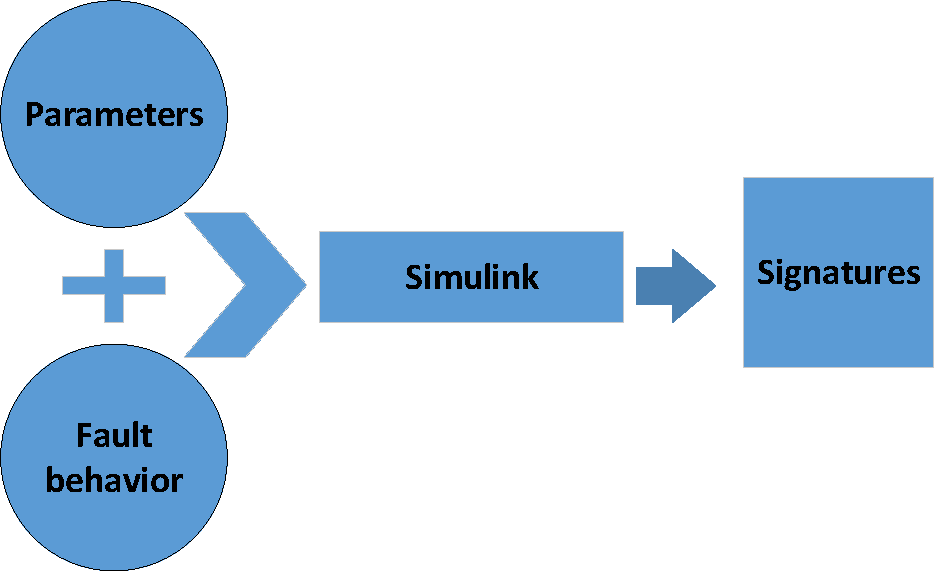
\includegraphics[scale=0.8]{Figures/fromhiddentosignature.pdf}
   \caption{Hidden states to Signatures}
\label{fig:HMMsig}
\end{figure}



 
\textbf{Example:} Consider an example of the signature and stuck-at-fault; an FPGA test designer can only sense the signature but wants to know the stuck-at-fault node to make the high-level model based on this information, i.e., hidden state. 

\textbf{Answer}: We will use the \underline{Viterbi Algorithm} to determine the most probable sequence of stuck-at-fault node by giving the sequence of signatures and HMM. Inshort, decoding helps to find the hidden sequence most likely to have generated a sequence of observation --- solved using Viterbi algorithm as shown in Figure~\ref{fig:HMMsig-Vit}.


\begin{figure}[tb!]

 \centering
  \captionsetup{justification=centering}    
   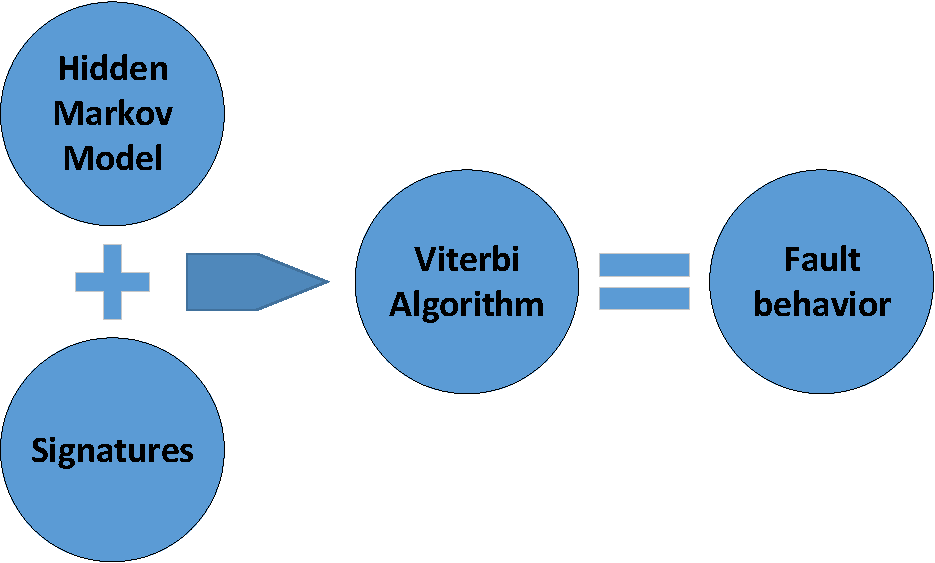
\includegraphics[scale=0.8]{Figures/HMM-plus-viterbi.pdf}
   \caption{Hidden states to Signatures}
\label{fig:HMMsig-Vit}
\end{figure}

\subsubsection{Viterbi Algorithm}


The Viterbi algorithm is based on the assumption that the most \textit{likely} path (hidden states sequence), $Q^* = argmax_Q P(Q|O) $, is a good estimation of the sequence of hidden states that generated the observed sequence $(O)$. The viterbi algorithm generates a path $X = (x_1, x_2,...,x_T)$, which is a sequence of states $x_n \in S = {s_1, s_2,...,s_k}$ that produce the sequence of observations $Y = (y_1,y_2,...,y_T) \in {1,2,...,N}^T N = Observation space$.

\textbf{Initialization:}



\begin{itemize}


\item The Observation space $O =  {o_1,o_2,...,o_N}$

\item the state space $S = {s_1,s_2,...,s_K}$

\item an array of the initial probabilities $\Pi = (\pi_1, \pi_2,...,\pi_K)$; $\pi_i is the probability the x_1 == s_i$

\item a sequence of observations $Y = (y_1,y_2,...,y_T)$; $yt == i$ the observation at time $t$ is $o_i$

\item the state transition matrix $A_ij$ stores the transition probability from state $s_i$ to $s_j$


\item emission matrix $B_ij$ stores the probability of observing $o_j$ from the state $s_i$
\end{itemize}  

\textbf{Recursion:}

We need to determine the hidden states by calculating $P(X|O)$. However, this brute force approach becomes intractable if the number of states gets larger, as the number of state path grows exponentially $(N^T)$. So, we need to calculate the $argmax_X P(X|O)$ . The most likely sequence is given by the recursion relations.

\begin{center}

\begin{itemize}


\item $V_1,k = P (y_1|k) \times \pi_k$

\item $V_t,k = max_{x \in S} (P (y_t|k) \times a_x,k \times V_t-1,x)$

\item $V_t,k$ probability of the most probably sequence $P (x_1, x_2,...,x_T, y_1,y_2,...,y_T)$

\end{itemize}

\end{center}


\textbf{Final:}

The most likely hidden state sequence $X = (x_1,x_2,...,x_N)$ 

\textbf{Example}


Consider you have an FPGA board, with some benchmark, e.g., counter is running on it. You need to  ask to perform a radiation induced experiment on it, drive the signatures, and make the high level model of it.

Suppose at any given time, the system can be in one of N possible states.

\begin{center}
$S = {S_1, S_2,....., S_N}$
\end{center}

From the experimental data you observed there are only three possible states in which system can go, e.g., stuck-at-1$\rightarrow O_{0}$, stuck-at-0$\rightarrow O_{1}$, and stuck-at-1$\rightarrow C_{1}$. I further observed that the transistion between these states can be described by the transition matrix.


\begin{center}


A = {$a_ij$} = \bordermatrix{~& & & \cr
                   & 0.4 & 0.3 & 0.3 \cr
                   & 0.2 & 0.6 &0.2 \cr
                   & 0.1 & 0.1 &0.8 \cr}
\end{center}

--- Question

\begin{itemize}
\item I model this behavior of the system in MATLAB and ask the high-level simulink designer you can find the response of the system as you like. He set the system paramters to know the faulty response of the system for the next seven different radiation experiment in order of (stuck-at-1$\rightarrow C_{1}$, stuck-at-1$\rightarrow C_{1}$, stuck-at-1$\rightarrow O_{0}$, stuck-at-1$\rightarrow O_{0}$, stuck-at-1$\rightarrow C_{1}$, stuck-at-0$\rightarrow O_{1}$, stuck-at-1$\rightarrow C_{1}$  ) given that the outcome of first radiation experiment is stuck-at-1$\rightarrow C_{1}$.

\item \textbf{Answer}


\item P(stuck-at-1$\rightarrow C_{1}$, stuck-at-1$\rightarrow C_{1}$, stuck-at-1$\rightarrow O_{0}$, stuck-at-1$\rightarrow O_{0}$, stuck-at-1$\rightarrow C_{1}$, stuck-at-0$\rightarrow O_{1}$, stuck-at-1$\rightarrow C_{1}$ | model)
\end{itemize}

\hspace{0.2cm} = P(stuck-at-1$\rightarrow C_{1}$) P(stuck-at-1$\rightarrow C_{1}$| stuck-at-1$\rightarrow C_{1}$) P(stuck-at-1$\rightarrow C_{1}$| stuck-at-1$\rightarrow C_{1}$) P(stuck-at-1$\rightarrow O_{0}$|stuck-at-1$\rightarrow C_{1}$) P(stuck-at-1$\rightarrow O_{0}$|stuck-at-1$\rightarrow O_{0}$) P(stuck-at-1$\rightarrow C_{1}$|stuck-at-1$\rightarrow O_{0}$) P(stuck-at-0$\rightarrow O_{1}$|stuck-at-1$\rightarrow C_{1}$) P(stuck-at-1$\rightarrow C_{1}$| stuck-at-0$\rightarrow O_{1}$)

\hspace{0.2cm} = $\pi_3$ $\times$ $a_33$ $\times$ $a_33$ $\times$ $a_13$ $\times$ $a_11$ $\times$ $a_31$ $\times$ $a_23$ $\times$ $a_32$

\hspace{0.2cm} = $1 \times 0.8 \times 0.8 \times 0.1 \times 0.4 \times 0.3 \times 0.1 \times 0.2$

The above mentioned model assumes that each state can be uniquely associated with an observable event. This model is too restrictive to be used for most of the realistic problems like ours, where we have no information of the underlying system only observe the outcome due to the result of change in hidden state.

\subsection{Learning}

The third application of the HMM is optimizing the parameters of the model. There are two possible solutions of this problem either to chose supervised learning and unsupervised learning.  In supervised learning you have one input variable, one output variable and use the algorithm to learn the mapping from the input to output, e.g., logistic regression, linear regression. We can map our problem to supervised learning, our goal is find the mapping function that when we have a new signature the mapping function can predict the stuck-at-node. Now, consider a case where I have only signature data and no information how these signatures comes from stuck-at-nodes.  This is the unsupervised learning because there is no answer available. In this thesis problem we opt for the unsupervised learning, because we have only the data available is signature, and we will find the parameters that maximize the probability of the hidden sequence.  

We can also find the optimal solution for our model by using the learning application of the HMM. The learning application works on the model parameters and observations to find the model that fits the data. There are three different techniques to do: a) Maximum Likelihood Estimation, b) Viterbi Training, and c) Baum  Welch = Forward-Backward Algorithm. 


Suppose we have a HMM: $\Pi = (\pi, A, B)$. The Baum-Welch algorithm is used to find  a local maximum for $\Pi^* = arg max_{\Pi} P (O | \Pi)$, i.e., the HMM parameters $\Pi$ that maximize the probability of the observation.

The Baum-Welch works in the following way:

\begin{enumerate}


\item Find the forward probabilities with the forward algorithm.


\begin{itemize}
\item $\alpha_{i}(1) = \pi_{i} b_{i} (o_{1})$
\item $\alpha_{i}(t + 1) = b_{i}(o_{t+1}) \sum\limits^{N}_{j=1}\alpha_{j}(t)a_{ji}$

\end{itemize}

\item Find the backward probabilities with the backward algorithm.

\begin{itemize}
\item $\beta(t) = P(o_{t+1} o_{t+2},...,o_{T} | x_{t} = i, \Pi) $

\item $\beta_{i}(T) = 1$
\item $\beta_{i}(t) = \sum\limits^{N}_{j=1} a[x_i, x_j] b[x_j,o_{t + 1}\beta_{j}(t + 1)]$

\end{itemize}
\item Find the probability of state $i$ at time $t$

\begin{itemize}

\item $P (x_t = i, O | \Pi) = P (o_1, o_2,...,o_t, x_t = i | \Pi) P (o_{t + 1}, o_{t + 2},...,o_{T} | x_{t} = i, \Pi) == \alpha_{i}(t) \beta_{i}(t) $

\item use the Bayes Theorem:

$P(x_t = i | O, \Pi) = \frac{P(x_t = i, O | \Pi)}{P(O | \Pi)} = \Upsilon_{i}(t)$

\end{itemize}
\item Find the probability of a transition from state $i$ to state $j$ at time $t$

\begin{itemize}
\item $\xi_{t}(i,j) = P (x_t = i,x_{t + 1} = j | O, \Pi)$


\item These probabilities can be computed bu using the forward and backward variables:

$\xi_{t}(i,j) = \frac{\alpha_i (t) a[x_i x_j] b[x_j,o_{t + 1}] \beta_j (t + 1)   }{P(O | \Pi)}$

\end{itemize}
\item Find the expected transition and emission counts:

$\sum\limits_{t = 1}^{ T } \Upsilon_i (t)$ = expected number of transition from $x_i$

$\sum\limits_{t = 1}^{ T} \xi_t (i ,j)$ = expected number of transition from $x_i$ to $x_j$

\item Perform the parameter estimation by the ratio of expected count the maximization step:


$\overline{a}[x_i, x_j] = \frac{\sum\limits_{t = 1}^{T - 1}\xi_{t} (i, j)}{\sum\limits_{t = 1} T - 1 \Upsilon_{j}(t)} $




$\overline{b}[x_i, o_k] = \frac{\sum\limits_{t = 1}^{T - 1}\Upsilon_{j} (t) 1 (o_t = k)}{\sum\limits_{t = 1}^{T - 1} \Upsilon_{j}(t)} $

\item Stop the computation when the change in the log likelihood is smaller than a given threshold or the maximum iterations are passed.

\end{enumerate} 















\section{High Level Error Analysis}








\section{Sequential Circuit Emulation}

%\subsection{Emulation Environment and Framework}
%\subsection{Sequential Circuit Fault Injection Mechanism}
%\subsection{Sequential Circuit Test Generation}


%\section{Modeling in Sequential Circuit}
%\subsection{Soft-Error Modeling and Analysis in Sequential Circuit}
%
%
%To analyze the faulty behavior of the sequential circuit by using Markov Chain theory is quite obvious choice. Markov chain analysis provide the steady state behavior of the sequential circuit. By using MC analysis we will able to find the number of clock cycles the sequential circuit produce the faulty output.
%
%As mentioned in the section related work, single error rate can be categorized into three different categories a)  circuit level b) gate level and c) architectural level.  Our work is focused on the architectural level by emulating the fault at circuit level. 




%Most of the real-time application of the electronic systems are sequential in nature, e.g., random access memories. A typical sequential circuit comprises of combinational logic and flip-flop as shown in Figure.   Inputs of the combinational logic, output of the combinational logic, and inputs and outputs of the flip-flop. There is a temporal correlations between the input signal and the state signal. The state signals are uniquely identified as the function of the input signal and the previous state signal. Due to this; sequential circuit error propagation from the error site, e.g., a bit flip in a flip-flop to the output can observe after several clock cycles. This temporal relationship force to use the more dynamic models than the models availble for the combinational circuits. The sequential circuits models can evolve with the time instances.
%
%We will make our faulty model from the real-time radiation experiment. We will start our analysis by analysing the faulty values. Let us consider the example of the counter as shown in Figure 1 fault free and Figure 2 faulty where output is stuck at 1 .  
%
%
%We will start our analysis by error probability matrix associated with the circuit and the probability that the erros comes in any part of the circuit (Combinational or flip-flop) produce an error at the output. 





%\section{Markov Chain Analysis for Faulty Behaviour Model}
%
%   
%
%
%
%
%$NS^{original}$ $=$  $\delta^{o}$ $=$ $(\delta^{o}_{1},\delta^{o}_{2},\delta^{o}_{3},...,\delta^{o}_{m})$
%
%
%$NS^{faulty}$ $=$  $\delta^{f}$ $=$ $(\delta^{f}_{1},\delta^{f}_{2},\delta^{f}_{3},...,\delta^{f}_{m})$
%
%
%$\delta^{o}$ $=$ Fault-Free circuit output values
%
%$\delta^{f}$ $=$ Faulty circuit output values
%
%$m$ $=$ Number of output variables
%
%From there I can construct my signature vector:
%
%
%$\epsilon_{signature}$ $=$ $\delta^{o}$  $-$ $\delta^{f}$
%
%
%Now, the main goal for the soft error analysis for sequential circuits is to find the transistion probabilities between the signatures from the signature vector $\epsilon_{signature}$ and from there to determine the faulty behaviour of the sequential circuits when soft-error occurs. 
%
%\subsection{SER Measurement in Sequential Circuits}
%
%\subsection{Modeling with Probabilistic Calculation Methods}

%\subsection{Modeling of Sequential Circuit with Markovian-Chain Analysis}



%The fault injection platform proposes for this project emulates SEUs, more specifically single-bit upsets (SBUs) within the configuration memory of SRAM-based FPGAs. We will study the effects of SEU on sequential circuits, and introduce a  framework for analyzing and detecting them. We will do the modeling and analysis of sequential circuits susceptibility to soft errors. Accurate sequential SEU estimation requires capturing the mechanism of error propagation and masking at both combinational and sequential levels. The challenging task for the sequential circuits under SEUs: the difference between sequential and combinational circuits from the context of ATPG and single stuck-at fault model. In this project, we will concentrate on sequential synchronous circuits. The problem we will face and encounter that the controllability of auxiliary inputs and observability of secondary outputs for the sequential circuits.  We will study and implement a technique which eases sequential circuits testing and ATPG by making controllability and observability much simple.
%
%\subsection{Fault Injection}
%
%We need to examine the behavior of a design under faults. For fault injection there are two strategies: (a) \textit{Software based fault injection}, and (b) \textit{FPGA based fault injection}. 
%
%\begin{itemize}
%
%\item Two methods will develop for software based fault injection. First, the source HDL code is modified to allow fault injection. Second, the simulation tool is used to force the error injection during simulation. 
%\item For FPGA-based simulation, we will use single error mitigation core from Xilinx~\cite{xilinx}. The idea is to integrate this core with our system to generate a modified bitstreams to emulate the occurrence of errors. We will use this strategy.
%\end{itemize}





%%\section{Research Axis 3: Radiation Bombardment}
%This part of the project is a neutron-induced Single Event Effect test in a commercial FPGA from Xilinx. The primary objective is to investigate the radiation effects reliability for the critical application. We will implement the sequential circuit and data acquisition system. The results we want to achieve to drive signatures for the sequential circuits. Our focus is on the analyzing the impact of multiple errors in state flip-flops, during the cycles following the cycle when faults occur. The following milestones we want to achieve from radiation bombardment experiment.
%
%\begin{itemize}
%\item Modeling of SEU, MBU and analyzing their effect on logic circuits.
%\item Evaluation of changes in error rates due to SEUs in sequential circuits.
%\item Compute the error probability, and signatures from bit-upsets can vary for different outputs and different circuits. 
%\item Evaluation of the impact of multiple flip-flop upsets in sequential circuits.
%\item Determining the outputs that are most susceptible to errors due to faults in logic.
%\item Determining the parts of the circuit (gates or gate clusters) that have the largest impact on circuit error probability.
%\item Estimation of lower and upper bounds of circuit susceptibility to transient.
%\end{itemize} 
%%
%\section{Research Axis 3: High-level Modelling}
%
%To model and analyze the sequential circuit susceptibility to soft errors, we need to used the approximate methods, e.g.,
%\begin{itemize}
%
%\item Binary Decision Diagram and Algebraic decision diagram.
%\item Markov-chain analysis based error rate estimation, which can provide steady-state Single-Error rate estimates following a hit. 
%\item A  Monte Carlo for SEU Analysis of Sequential Circuits based on the probability of the bit-flips and estimates the states outputs and signatures.
%
%\end{itemize}
%\subsection{Simulator}
%
%We also have a plan to develop a simulator with the help of \textit{isoneo}. The simulator is based on the Matlab / Simulink models. The simulator takes the input a parameterization file corresponding to the operational architecture of the system. This file is generated from the configurator; it is in XML format.
%From this configuration, the simulator initially initializes a model of the system failure tree.
%This model is then exploited dynamically during the simulation phase to evaluate the level of reliability of the system and its components. The simulator executes the simulation model with the constraints and concludes a level of safety for each equipment and the global system.

%\section{Optional: Fault Mitigation}
%Fault-mitigation can be achieved in two ways: preventing faults from happening and
%recovering after their occurrence. Fault preventing is achieved by using hardened components and/or shielding. But fault preventative is not a viable solution in terms of a project cost. More complex fault-mitigation methodologies can be implemented at the architectural level. We need to develop some fault-mitigation strategies like triple module redundancy with  dynamic reconfiguration of the hardware~\cite{jacobs2012reconfigurable} and/or something like the work presented in 
%%Jacobs \emph{et al.}~\cite{jacobs2012reconfigurable} and Alderighi \emph{et al.}~\cite{violante} promote the use of SRAM-FPGAs for reconfigurable fault-tolerant space applications.
%~\cite{jacobs2012reconfigurable} used fault tolerance framework (RFT) that enables system designers to dynamically adjust a system's level of redundancy and fault mitigation based on the varying radiation incurred at different orbital positions. Notably, the reconfigurable fault tolerance framework in~\cite{jacobs2012reconfigurable} is based on an upset rate modeling tool that used to capture time-varying radiation effects in a given orbit.


\section{Project Plan}


\textbf{Summary}

\textbf{Phase  01:} The emulation platform will be the starting point of research. We will use the SEUs for the configuration memory upsets. Selection of a suitable benchmark, which is probably ITC'99~\cite{ITC}used for the testing purpose and signature generation.

\textbf{Phase  02:} Evaluate the radiation based experimental setup results for signature under the neutron radiation at Triumf.


\textbf{Phase 03:} Implement that above mentioned methodology and high-level model for soft-error of sequential circuits.

%\section{Timetable}
%The development of the tasks identified in Chapter~\ref{sec:approach}, and the most important milestones of this project are presented in Figure~\ref{timetable}.
%In our intentions, the design of a time predictable computer architecture, the development of novel timing analysis techniques, and the FPGA prototypes implementation will unfold as a series of sequential tasks with relatively small interleaving. Dependability and real-time requirements, on the other hand, should be kept in mind throughout the whole advancement of the project.

\begin{figure}[h]
\centering
\begin{tikzpicture}
\begin{ganttchart}[
x unit=0.36cm,
y unit title=1.0cm,
y unit chart=1.5cm,
%vgrid,
hgrid,
inline,
]{1}{48}
\gantttitle{Research Project}{48} \\
\gantttitle{2016}{12} \gantttitle{2017}{12} \gantttitle{2018}{12} \gantttitle{2019}{12}\\



\ganttbar[bar height=.4]{Literature Review and Comp .Exam}{6}{24}\\
%\ganttmilestone[]{Comp. Exam}{20}\\
%\ganttmilestone[]{AHS}{6}
%\ganttmilestone[]{TODAES}{12}\\
\ganttbar[bar height=.4]{Emulation Platform for Seq. ckt}{6}{35} \\
\ganttbar[bar height=.4]{Radiation Experiment}{13}{24} \\
\ganttbar[bar height=.4]{Modelling and Simulator}{25}{42} \\
%\ganttmilestone[]{TAAS}{30}\\
%\ganttbar[bar height=.4]{Novel Timing analysis techniques}{22}{38} \\
%\ganttmilestone[]{DAC}{36}\\
%\ganttbar[bar height=.4]{FPGA Implementation}{27}{38} \\
%\ganttmilestone[]{TRETS}{40}\\
\ganttbar[bar height=.4]{Tech. Demo.}{35}{42} \\
%\ganttmilestone[]{IAC}{44}\\
\ganttbar[bar height=.4]{Thesis Writing}{35}{46}
%\ganttmilestone[]{Thesis}{44}\\
%\ganttbar[bar height=.4]{The \emph{PolyOrbite} Project}{1}{44} 

%\ganttlink{elem0}{elem1}
%\ganttlink{elem0}{elem2}
%\ganttlink{elem0}{elem3}

%\ganttlink{elem3}{elem4}

%\ganttlink{elem5}{elem6}
%\ganttlink{elem5}{elem7}

%\ganttlink{elem7}{elem8}
\end{ganttchart}
\end{tikzpicture}
\caption{Timetable.}
\label{timetable}
\end{figure}












\chapter{Preliminary Results}


In this chapter, we present the preliminary results of this research work. The work I have done so far. These results are focused on the three things a) relative sensitivity based emulation, b) High-level fault model for adder and multiplier\footnote{Mr. Claude thibeault performed the experiment using Tesssent }, c) sequential circuit signature generation.



\section{A new Emulation Technique Based on Bits Relative Sensitivity
for SRAM FPGAs}
\label{intro}
% no \IEEEPARstart

The purpose of this work is to  studying the relative sensitivity ratio difference between the configuration bits set to "1" and those set to "0" to produce the highly accurate fault behavior as expected in the real-time testing environment. Because the work is done in~\citep{souari2016towards}, showed that if we considered the bits relative sensitivity difference, i.e., the bits at "1" are more sensitive than the bits at "0", meaning, bits set to "1" are more likely to generate faults than the bits set at "0". We get more realistic results, closer to the radiation-based experiments based on this theory. 
In this work, the new fault emulation technique is introduced which based on the bits relative sensitivity, and its features, i.e., bits set to "1" or "0" plus the bit either belongs to LUT or non LUT bits.  We observed that the signature computed by relative sensitivity-based method is $97.8$\% closer to adder circuit signature and $99.4$ \% closer to multiplier circuit signature observed from the radiation based experiment.
This work is the extension of the previous work and make the following contributions. 

\textbf{Contributions:} 
\begin{itemize}

\item{Developed a realistic fault emulation technique in the configuration memory
of FPGAs based system}.
\item{In this work, we propose a fault injection method by using relative sensitivity values between the bits features: e.g., bits belong to LUT at "0", bits belong to LUT at "1", bits belong to Non-LUT at "0", bits belong to Non-LUT at "1"}.
\item{Zero-signature has been derived by flipping the bits-at-1, bits-at-0, randomly, flipped the bits based on the relative sensitivity between bits-at-1, bits-at-0, and relative sensitivity between bits-status and their features}.
\end{itemize}


\section{Methodology}
\label{Methodology}
The emulation of SEUs in an FPGA is done by flipping the bit in the configuration memory by using the IP provided by the Xilinx named - SEM core~\citep{xilinx}. The emulation platform used in this work was designed for the radiation experiment~\citep{hobeika2014multi}. In this work, this platform is employed for the fault emulation. The platform comprises of two Artix-7 FPGAs. The "Reference-Board" comprises of the original design, e.g., 16-bit adder and 8-bit multiplier. The design under "Test-Board" is subjected to fault emulation.  

\subsection{Identification of the Sensitivity bits}
\label{SE-bits}
The first step is the identification of the bits (the bit address and the bit location). The identification of the bits is important in our work because we want to emulate such a fault injection experiment that produce the same result as expected in the real experiment.
I develop some tools that extract the bit address and the bit location from the .rbd file of the design. The \textit{.rbd} an ASCII file that contains readback data, including pad words and frames.
The proposed procedure is shown in Figure~\ref{fig:original-rbd}, and Figure~\ref{fig:inverted-rbd}.  I used two tools for this purpose: 
\begin{itemize}
\item Xilinx ISE tool to generate the .ncd file and .xdl file of the design that helps to find the bits feature which bits belongs to LUT and which are non-LUT bits.
\item I used Vivado tool to get the .rbd file of the design from the FPGA.

\item 
\end{itemize}

The classification of the bits comprises consists of following steps:
\begin{itemize}
\item Generate the \textit{.ncd} file of the design, generate the original \textit{.bit} file, downloaded it into the FPGA and used the vivado \textit{readback} command to read the original \textit{.rbd} file.
\item Then from the \textit{.ncd} file of the design generate the \textit{.xdl} file of the design  which contains placement information of primitive sites, and their routing regarding switch matrix connections.
\item Python script has been developed that inverts all the logic of LUTs in the .xdl file, and generates the modified \textit{.ncd} file, and modified \textit{.bit} file as shown in Figure~\ref{fig:inverted-rbd}.
\item Once we get both two files, we further investigated to find the bits features that which bits belong to the LUTs and which are non-LUTs bits.
\item Algorithm~\ref{BCA} describe the feature extraction procedure. For example, if the bit is at state "one" in the original .rbd file and it's being detected "zero" in the inverted .rbd file means bit belongs to the LUT bits at "one" represented as (L1)." Similarly, for non-lut-at-0 (NL0), non-lut-at-1 (NL1), and lut-at-0 (L0). 
\end{itemize}

\begin{figure}[tb!]
 \centering
  \captionsetup{justification=centering}    
   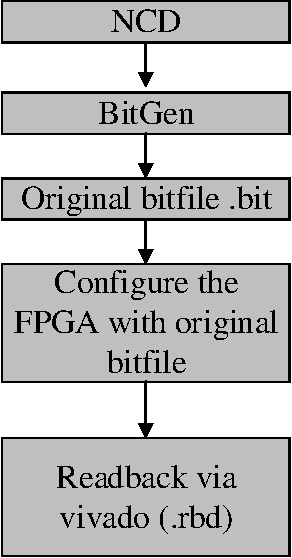
\includegraphics[scale = 0.5]{Figures/original-rbd.pdf}
   \caption{Procedure to extract the original .rbd file}
\label{fig:original-rbd}
\end{figure}
\begin{figure}[tb!]
 \centering
  \captionsetup{justification=centering}    
   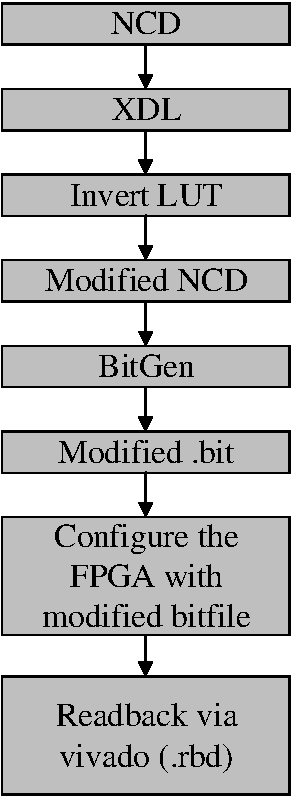
\includegraphics[scale = 0.5]{Figures/inverted-rbd.pdf}
   \caption{Procedure to extract the inverted LUT .rbd file}
\label{fig:inverted-rbd}
\end{figure}


\begin{algorithm}
\caption{Bits classification algorithm.}
\begin{algorithmic}
\label{BCA}
\REQUIRE $.rbd$ $original$ $and$ $.rbd$ $inverted$ \\
%\textbf{Compute}\\ 
%\hspace{1.5cm}{$Original =  A $ $ \times $ $ B$ } \\
%\hspace{1.5cm}{$Faulty =  A $ $ \times $ $ B$ } \\
%\vspace{0.20 cm }
%\textbf{Stuck-at-1:}
\vspace{0.20 cm }
\IF{$Original$  $ = $ $ 0 $  $Inverted$ $==$ $0$}
\vspace{0.10 cm }
\STATE \textit{ NL0 = Not LUT bits at 0}
\vspace{0.10 cm }
\ELSIF{$Original$  $ = $ $ 0 $  $Inverted$ $==$ $1$}
\vspace{0.10 cm }
\STATE \textit{ L0 = LUT bits at 0}
\vspace{0.10 cm }
\ELSIF{$Original$  $ = $ $ 1 $  $Inverted$ $==$ $0$}
\vspace{0.10 cm }
\STATE \textit{ L1 =  LUT bits at 1}
\vspace{0.10 cm }
\ELSIF{$Original$  $ = $ $ 1 $  $Inverted$ $==$ $1$}
\vspace{0.10 cm }
\STATE \textit{ NL1 = Not LUT bits at 1}
\vspace{0.10 cm }


\ENDIF
\vspace{0.20 cm }
\end{algorithmic}
\end{algorithm}



\section{Experimental Results}
\label{Experimental Results}
In this section, we will discuss the result of emulation performed by flipping the bits at "1" and at "0." We experimented with fifty different runs. Each run provides $6,144$ signatures further subdivided into three different groups. 
Table~\ref{AE}, and Table~\ref{ME} show the percentage of the zero signatures, e.g., $00000000$ for adder and multiplier. The maximum number of zero signatures observed for flip-at-0. The number of bits flipped observed; $65,750$ among them $150$ bits are critical bits with the statistical ratio of $0.22\%$ critical bits at $0$. The minimum number of zero signatures observed for bits flip-at-1, with the total flipped bits are $1,356$ among $3,110,418$ non-BRAM bits. In this case, the critical bits at $1$ are $11.06\%$. 
Similarly, for the multiplier,  the number of bits flipped observed are $29,752$ with total non-BRAM(bits-at-0) are $56,771,430$ giving the statistical ratio of $0.50\%$ critical bits at $0$. The minimum number of zero signatures observed for bits flip-at-1, with the total flipped bits are $1,664$ among $3,750,970$ non-BRAM bits. In this case, the critical bits at $1$ are $9.01\%$.

Then the emulation performed with the random fault injection, in which we randomly combined the bits-at-1, and the bits-at-0 and calculated the zero signatures. As expected, the random injection zero-signature value should lower than the flip-at-0 and higher than the flip-at-1 because the number of bits at "0" are $18.45$ times higher than the bits at "1" for adder and  $15.13$ for multiplier. The purpose of performing the random injection is to compare the result with the relative sensitivity results and experimentally prove that by considering the relative sensitivity of the bits more realistic results are produced. The bit flip ratio observed in the random injection (flip-at-0 to flip-at-1) is $18.10$ for the adder as shown in Table~\ref{RI} and $15.15$ for the multiplier as shown in Table\ref{RIM}. This bit-flip information indicates that the bit flip in random mode is valid. Next, we performed the relative sensitivity experiment named SA-01, and SA-02.
In SA-01, we used the relative sensitivity concept that the  bits-at-1 are $2.11$ times more sensitive than the bit-at-0. In this emulation, we get the $7.95\%$ difference with the irradiation experiment for the adder and $1.58\%$ for the multiplier. The total bit flips we observed for adder are: $9,807$ among them $8,797$ flipped-at-0 and $1,010$ for flipped-at-1. Similarly, for the multiplier, the total bits flipped are $7,227$ among them $6,345$ flipped-at-0 and $882$ flipped-at-1. Both emulation gives us a bit flipped ratio of $2.11$ proved that emulation setup is valid. 





\begin{table}[tb!]
\center
\caption{Adder Emulation Tests Comparison.}
\label{AE}
\begin{tabular}{|c | c| c | c| c| c |} 
 \hline
Test & Zero Signature (\%) & Difference with Radiation (\%)   \\ 
\hline
 
 
 Flip@1& 49.0 &22.53   \\
 \hline
 Flip@0 & 62.8 & 2.25 \\ 
 \hline
 
 Random & 58.1 & 5.52  \\
 \hline
 SA-01 & 56.7 & 7.95 \\
 \hline
 SA-02 & 60.16 & 2.13  \\
 \hline
 Radiation & 61.4 & 0  \\
 \hline
 
 
\end{tabular}
\end{table}

\begin{table}[tb!]
\center
\caption{Multiplier Emulation Tests Comparison.}
\label{ME}
\begin{tabular}{|c | c| c | c| c| c |} 
 \hline
Test & Zero Signature (\%) & Difference with Radiation (\%)   \\ 
\hline
 
 
 Flip@1& 62.0 &18.35   \\
 \hline
 Flip@0 & 76.0 & 1.93 \\ 
 \hline
 
 Random & 72.1 & 3.31  \\
 \hline
 SA-01 & 73.4 & 1.58 \\
 \hline
 SA-02 & 74.9 &  0.50\\
 \hline
 Radiation & 74.6 & 0  \\
 \hline
 
 
\end{tabular}
\end{table}



\begin{table}[tb!]
\center
\caption{Adder Random Injection Bits Information.}
\label{RI}
\begin{tabular}{c c  c c   } 
 \hline
\multicolumn{2}{c}{Bit}     & Flip Ratio (Theoretical) &  Flip Ratio (Observed)   \\ 
%\hline
%& \multicolumn{1}{c}{ (Theoretical)} \\
%& & \multicolumn{1}{c}{observed} \\
 \hline
 
 Bits@0 & $57 411 982  $ & \multirow{2}{*}{18.45} & \multirow{2}{*}{18.10} \\
 %\hline
 Bits@1 & $3110418$  & &\\ 
 \hline
% 
% Bits@0 LUT & 2.06 &2.08 &2.096\\
% \hline
% Bits@1 LUT & 1.91 &1.92&1.91\\
 %\hline
% \hline
 
 
\end{tabular}
\end{table}

\begin{table}[tb!]
\center
\caption{Multiplier Random Injection Bits Information.}
\label{RIM}
\begin{tabular}{c c  c c   } 
 \hline
\multicolumn{2}{c}{Bit}     & Flip Ratio (Theoretical) &  Flip Ratio (Observed)   \\ 
%\hline
%& \multicolumn{1}{c}{ (Theoretical)} \\
%& & \multicolumn{1}{c}{observed} \\
 \hline
 
 Bits@0 & $57 411 982  $ & \multirow{2}{*}{15.93} & \multirow{2}{*}{15.15} \\
 %\hline
 Bits@1 & $3110418$  & &\\ 
 \hline
% 
% Bits@0 LUT & 2.06 &2.08 &2.096\\
% \hline
% Bits@1 LUT & 1.91 &1.92&1.91\\
 %\hline
% \hline
 
 
\end{tabular}
\end{table}


Then, we further investigated the bits feature, i.e., bits belong to LUT and non-LUT bits. We used the bits relative sensitivity values shown in Table~\ref{RS}. The result we obtained by using this approach indicates only $2.13\%$ difference for adder and $0.50\%$ for multiplier suggests that by considering bits sensitivity with bits features more realistic results can be achieved, and better fault emulation can be performed. 

%\begin{table}[tb!]
%\center
%\caption{Adder Emulation Tests Comparison.}
%
%\label{AE}
%
%\begin{tabular}{|c | c| c | c| c| c |} 
% \hline
%Test & Zero Signature (\%) & Difference with Radiation (\%)   \\ 
%\hline
%
% 
% 
% Flip@1& 49.048 &22.53   \\
% \hline
% Flip@0 & 62.801 & 2.095 \\ 
% \hline
% 
% Random & 59.378 & 3.51  \\
% \hline
% SA-01 & 60.36 & 1.87 \\
% \hline
% SA-02 & 60.559 &1.47  \\
% \hline
% Radiation & 61.499 & 0  \\
% \hline
% 
% 
%\end{tabular}
%\end{table}


We also measure the relative sensitivity (observed) and the bit flip information observed for this emulation setup shown in the Table~\ref{RS} to prove the bit flip emulation validity. Table~\ref{RSflipA} and~\ref{RSflipM} shows the bit flip information for the adder and multiplier respectively.

\begin{table}[tb!]
\center
\caption{Relative Sensitivity from experimentation performed at TRIUMF.}
\label{RS}
\begin{tabular}{|c | c| c | c | } 
 \hline
Bits feature & \makecell*{Relative Sensitivity}  & \makecell*{Adder \\(Observed)} & \makecell*{Multiplier \\ (Observed)}  \\ 
%\hline
%& \multicolumn{1}{c}{ (Theoretical)} \\
%& & \multicolumn{1}{c}{observed} \\
 \hline
 
 Bits@0 non LUT & 1.00 & 1.00 & 1.00 \\
 \hline
 Bits@1 non LUT& 1.41  & 1.43&1.44\\ 
 \hline
 
 Bits@0 LUT & 2.06 &2.08 &2.09\\
 \hline
 Bits@1 LUT & 1.91 &1.92&1.91\\
 \hline
% \hline
 
 
\end{tabular}
\end{table}









\begin{table}[tb!]
\center
\caption{Bit Flip Ratio Relative Sensitivity (Adder).}
\label{RSflipA}
\begin{tabular}{|c | c| c | c | } 
 \hline
Bits feature & \makecell*{Bit Flip)}  & \makecell*{Bit Flip Ratio\\(Total)} \\ 
%\hline
%& \multicolumn{1}{c}{ (Theoretical)} \\
%& & \multicolumn{1}{c}{observed} \\
 \hline
 
 Bits@0 non LUT & 5251  & 1.00  \\
 \hline
 Bits@1 non LUT& 236  & 1.43\\ 
 \hline
 
 Bits@0 LUT & 266 &2.08 \\
 \hline
 Bits@1 LUT & 245 &1.92\\
 \hline
% \hline
 
 
\end{tabular}
\end{table}

\begin{table}[tb!]
\center
\caption{Bit Flip Ratio Relative Sensitivity (Mull).}
\label{RSflipM}
\begin{tabular}{|c | c| c | c | } 
 \hline
Bits feature & \makecell*{Bit Flip}  & \makecell*{Bit Flip Ratio\\(Total)} \\ 
%\hline
%& \multicolumn{1}{c}{ (Theoretical)} \\
%& & \multicolumn{1}{c}{observed} \\
 \hline
 
 Bits@0 non LUT & 8833  & 1.00  \\
 \hline
 Bits@1 non LUT& 454  & 454\\ 
 \hline
 
 Bits@0 LUT & 603 &2.09\\
 \hline
 Bits@1 LUT & 553 &1.91\\
 \hline
% \hline
 
 
\end{tabular}
\end{table}


\section{Conclusions}

In this work, sensitivity of the configuration bits has been considered along with the bits feature to
produce results as close as possible to those obtained by the accelerated tests. 

\label{Conclusion}
%
%\chapter{Conclusion}
% 

In this proposal, we have demonstrated our research will be focused on investigation of a design, methodologies, and implementation of a time predictable fault tolerant computing system evaluated by the probabilistic timing analysis (PTA). As our target domain is a real-time industry. We will stress the importance of a worst case execution time (WCET) estimation.
Nowadays, the investigations of new timing analysis techniques are an unavoidable need because of the growing complexity of a modern embedded computers and the aerospace industry will especially a benefit from the introduction of a such technologies in terms of  reliability and design costs. Our approach will leverage probabilistic approach to enable the timing analysis in computing systems.
As a consequence, this research has a potential to make computing systems smarter, more reliable, and easier to design and to program. At the same time, we think that our results will make decisive steps ahead in a fairly unexplored research area - integration of fault-tolerance techniques in time predictable computer architecture.


In our preliminary results, we showed that how probabilistically analysable cache can be integrated in a MIPS processor to make the foundation for a probabilistically analysable computing systems. The research published in~\cite{NEWCAS} proved the effectiveness of a measurement based probabilistic timing analysis (MBPTA). Furthermore, our most recent results demonstrated that probabilistic timing technique is a promising approach for the future timing analysis of a real-time aerospace embedded system.

Through this research, we hope to be able to have an impact on how computer engineers and system designers will think of probabilistic computing in near future, and contribute to create the next generation of a real-time embedded systems for aerospace industry.
We will target field-specific international  journals such as the ``ACM Transactions on Real-time  Systems'' and the ``ACM Transactions on Reconfigurable Technology and Systems'', or conferences including tracks dedicated to the automated design of embedded systems, such as the ``Design Automation Conference'' and the ``Design, Automation \& Test in Europe'' conference.

\section{Work Breakdown Structure}
Figure~\ref{wbs} presents the work breakdown structure (WBS) of our research project. At level 2 of this tree chart, we identify four groups of tasks: the ones related to the acquisition of knowledge; those related to the development of new knowledge; an experimental phase; and, finally, project management tasks.

Knowledge acquisition includes the class work done towards the credit requirements of the PhD program and the review of the scientific literature. 

The knowledge extension task can be split along the four research axes defined in Chapter~\ref{sec:approach}. The experimental phase goes from the definition of a test plan to the experimental evaluation of our prototype on a CubeSat  platform.

Project management tasks involve the writing of conference and journal articles, as well as the preparation of a thesis and its defense.

\begin{figure}[h]
\vspace{2cm}
\centering
\begin{tikzpicture}[
  level 1/.style={sibling distance=40mm},
  edge from parent/.style={->,draw},
  >=latex]

% root of the the initial tree, level 1
\node[root, fill = black!30] {Research Project}
% The first level, as children of the initial tree
  child {node[level 2,fill = black!10] (c1) {Knowledge Acquisition}}
  child {node[level 2,fill = black!10] (c2) {Knowledge Extension}}
  child {node[ level 2,fill = black!10] (c3) {Experimental Phase}}
  child {node[level 2,fill = black!10] (c4) {Project\\ Management}};

% The second level, relatively positioned nodes
\begin{scope}[every node/.style={level 3}]
\node [rounded corners,fill = white, below of = c1, xshift=15pt] (c11) {\footnotesize Classes};
\node [rounded corners,fill = white, below of = c11] (c12) {\footnotesize Literature\\ Review};

\node [rounded corners,fill = white, below of = c2, xshift=15pt] (c21) {\footnotesize PTA};
\node [rounded corners,fill = white, below of = c21] (c22) {{\footnotesize Predictable computing}};
\node [rounded corners,fill = white, below of = c22] (c23) {\footnotesize Fault tolerance};
\node [rounded corners,fill = white, below of = c23] (c24) {\footnotesize Reconfiguration.};
\node [rounded corners,fill = white, below of = c24] (c25) {\footnotesize Multicore Architecture.};

\node [rounded corners,fill = white, below of = c3, xshift=15pt] (c31) {\footnotesize Design};
\node [rounded corners,fill = white, below of = c31] (c32) {\footnotesize Algorithm Eval.};
\node [rounded corners,fill = white, below of = c32] (c33) {\footnotesize FPGA Implementation.};
\node [rounded corners,fill = white, below of = c33] (c34) {\footnotesize Tech. Demo.};

\node [rounded corners,fill = white, below of = c4, xshift=15pt] (c41) {\footnotesize Conferences};
\node [rounded corners,fill = white, below of = c41] (c42) {\footnotesize Journals};
\node [rounded corners,fill = white, below of = c42] (c43) { \footnotesize Thesis and\\ Graduation};
%\node [fill = black!30, below of = c43] (c44) {Thesis and\\ Graduation};

\end{scope}

% lines from each level 1 node to every one of its "children"
\foreach \value in {1,2}
  \draw[->] (c1.195) |- (c1\value.west);

\foreach \value in {1,...,5}
  \draw[->] (c2.195) |- (c2\value.west);

\foreach \value in {1,...,4}
  \draw[->] (c3.195) |- (c3\value.west);

\foreach \value in {1,...,3}
  \draw[->] (c4.195) |- (c4\value.west);
\end{tikzpicture}
\caption{Work breakdown structure.}
\label{wbs}
\end{figure}

\newpage
\section{Timetable}
The development of the tasks identified in Chapter~\ref{sec:approach}, and the most important milestones of this project are presented in Figure~\ref{timetable}.
In our intentions, the design of a time predictable computer architecture, the development of novel timing analysis techniques, and the FPGA prototypes implementation will unfold as a series of sequential tasks with relatively small interleaving. Dependability and real-time requirements, on the other hand, should be kept in mind throughout the whole advancement of the project.

\begin{figure}[h]
\centering
\begin{tikzpicture}
\begin{ganttchart}[
x unit=0.36cm,
y unit title=1.0cm,
y unit chart=1.5cm,
%vgrid,
hgrid,
inline,
]{1}{48}
\gantttitle{Research Project}{48} \\
\gantttitle{2015}{12} \gantttitle{2015}{12} \gantttitle{2016}{12} \gantttitle{2017}{12}\\



\ganttbar[bar height=.4]{Literature Review}{1}{16}\\
%\ganttmilestone[]{Comp. Exam}{20}\\
%\ganttmilestone[]{AHS}{6}
%\ganttmilestone[]{TODAES}{12}\\
\ganttbar[bar height=.4]{Leon 3 processor analysis}{13}{32} \\
\ganttbar[bar height=.4]{Architectural Modifications}{17}{32} \\
\ganttbar[bar height=.4]{Probabilistic component design}{18}{38} \\
%\ganttmilestone[]{TAAS}{30}\\
\ganttbar[bar height=.4]{Novel Timing analysis techniques}{22}{38} \\
%\ganttmilestone[]{DAC}{36}\\
\ganttbar[bar height=.4]{FPGA Implementation}{27}{38} \\
%\ganttmilestone[]{TRETS}{40}\\
\ganttbar[bar height=.4]{Tech. Demo.}{35}{42} \\
%\ganttmilestone[]{IAC}{44}\\
\ganttbar[bar height=.4]{Thesis Writing}{35}{46}
%\ganttmilestone[]{Thesis}{44}\\
%\ganttbar[bar height=.4]{The \emph{PolyOrbite} Project}{1}{44} 

%\ganttlink{elem0}{elem1}
%\ganttlink{elem0}{elem2}
%\ganttlink{elem0}{elem3}

%\ganttlink{elem3}{elem4}

%\ganttlink{elem5}{elem6}
%\ganttlink{elem5}{elem7}

%\ganttlink{elem7}{elem8}
\end{ganttchart}
\end{tikzpicture}
\caption{Timetable.}
\label{timetable}
\end{figure}





%%%
%%%  SYNTHESE DES TRAVAUX
%%%
%\section{Synthèse des travaux}
%Texte.
%
%%%
%%%  LIMITATIONS
%%%
%\section{Limitations de la solution proposée}\label{sec:Limitations}
%
%%%
%%%  AMELIORATIONS FUTURES
%%%
%\section{Améliorations futures}
%Texte.



%\section{Layout tests}

%In this sections, several environments are presented.
%
%\subsection{Listing tests}
%
%Presentation of the main listing environments: enumerations and lists.
%
%\subsubsection{Enumerations: enum environment}
%
%Enum environment test:
%\begin{enumerate}
% \item test 1
% \item test 2
%\end{enumerate}
%
%\subsubsection{Lists: itemize environment}
%
%Test of the itemize environment
%\begin{itemize}
% \item test 1
% \item test 2
%\end{itemize}
%
%\subsection{Equations tests}
%
%Layout of the equations:
%
%\begin{equation}
%   \beta = 8
%\end{equation}
%
%\begin{equation}
%   \gamma = \alpha \times 3
%\end{equation}
%
%\section{Second section}
%
%Example of a second section, to test the layout in the table of contents.
%
%
%%%- Second demo chapter -%%
%\chapter{Second Chapter}
%
%\section{Table layout tests}
%
%Tables have the same constraints than the figures, except for the caption that has to be on top.
%
%
%\begin{table}
%		\parbox{0.65\textwidth}{\caption{Test of a long table caption, with linebreak.}} % Contrainte manuelle de la largeur de la légende
%		\begin{tabular}{|c|c|c|c|c|c|c|c|}
%		\hline
%			{\bf titre} & {\bf titre} & {\bf titre} & {\bf titre} & {\bf titre} & {\bf titre} & {\bf titre} & {\bf titre} \\
%	  \hline
%			blá & blá & blá & blá & blá & blá & blá & blá \\
%	  \hline
%			blá & blá & blá & blá & blá & blá & blá & blá \\
%	  \hline
%			blá & blá & blá & blá & blá & blá & blá & blá \\
%	  \hline
%			blá & blá & blá & blá & blá & blá & blá & blá \\
%	  \hline
%			blá & blá & blá & blá & blá & blá & blá & blá \\
%	  \hline
%			blá & blá & blá & blá & blá & blá & blá & blá \\
%	  \hline
%		\end{tabular}
%\end{table}
%
%
%\section{References test}
%
%\subsection{References to the bibliography}
%
%Reference from the bibliography \cite{BookExample}.
%
%\subsection{References to the list of references "refs"}
%
%References from the list of references "refs", declared at the beginning of the document \citerefs{Test}.
%
%\subsection{References to a label of the document}
%
%Reference to a Figure associated to a label: Figure \ref{fig:vueEts}.
%
%\subsection{URL references}
%
%\subsubsection{Test of "href"}
%
%Href is used to integrate a link to a text:
%\href{http://www.etsmtl.ca/Etudiants-actuels/Cycles-sup/Realisation-etudes/Guides-gabarits}{Link to the template page.}.
%
%\subsubsection{Test de url}
%
%Url is used to format a clickable link:
%\url{http://www.etsmtl.ca/Etudiants-actuels/Cycles-sup/Realisation-etudes/Guides-gabarits}.
%
%%%- Third demo chapter -%%
%\chapter{Example of a thesis by article, with integrated article}
%
%% \articleAuthors{Names}{Affiliations} is used to print authors and their affiliations. Names must be declared as {First name1 Last Name1}{First Name2 Last Name2}... , as well as the affiliations
%%Exemple \articleAuthors{{First Name Last Name}}{{Affiliation}}
%
%\articleAuthors{
%{First name Last name\textsuperscript{1}}{First name Last name\textsuperscript{1}}
%}{
%{\textsuperscript{1} Département de Génie Mécanique, École de Technologie Supérieure,\\
%1100 Notre-Dame Ouest, Montréal, Québec, Canada H3C 1K3
%\\~\\
%Article soumis à la revue « Vecteur environnement » en septembre 2010.}
%}
%
%\section{Section 1}
%
%\lipsum[1] % Text filling, to have an example of the layout
%
%%%- Conclusion -%%
%\begin{conclusion}
%
%\lipsum[1] % Text filling, to have an example of the layout
%
%\end{conclusion}
%



%%%%%%%%%%%%%%%%%%%%%%%%%%%%%%%%%%%%%%%%%%%%%%%%%%%%
%%  Appendix example:
%%%%%%%%%%%%%%%%%%%%%%%%%%%%%%%%%%%%%%%%%%%%%%%%%%%%
%\appendix
%
%%% To use more than one appendix
%\multiannexe
%
%%% Appendix from an external file
%% \include{extApp}

\chapter{Appendix example}


\section{First section of the appendix}


\subsection{Figures in annexes}

%\begin{figure}
%	\centering
%	\fbox{
%		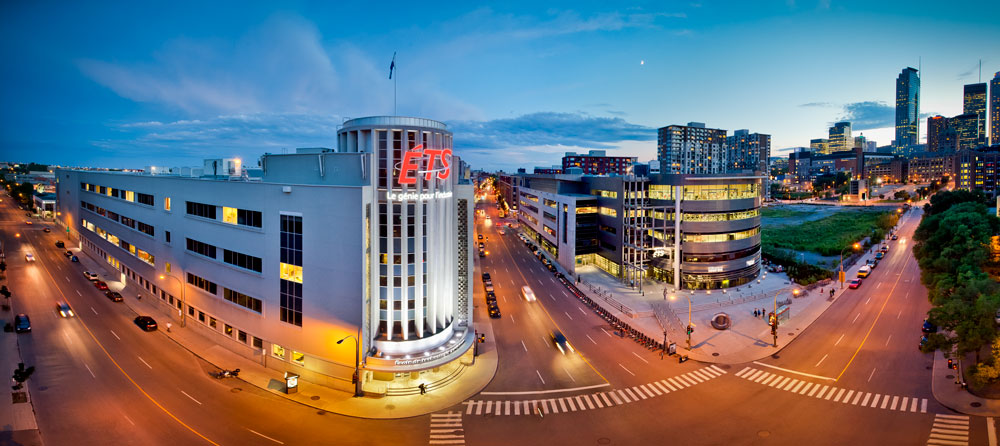
\includegraphics[width=0.75\textwidth]{Figures/vueEts.jpg}
%	}
%	 \\ \parbox{0.75\textwidth}{\caption{Figure in an appendix.}\label{fig:testAp}}
%\end{figure}
%
%\begin{figure}
%	\centering
%	\fbox{
%	\parbox{0.975\linewidth}{
%	\subfloat[first figure]{
%		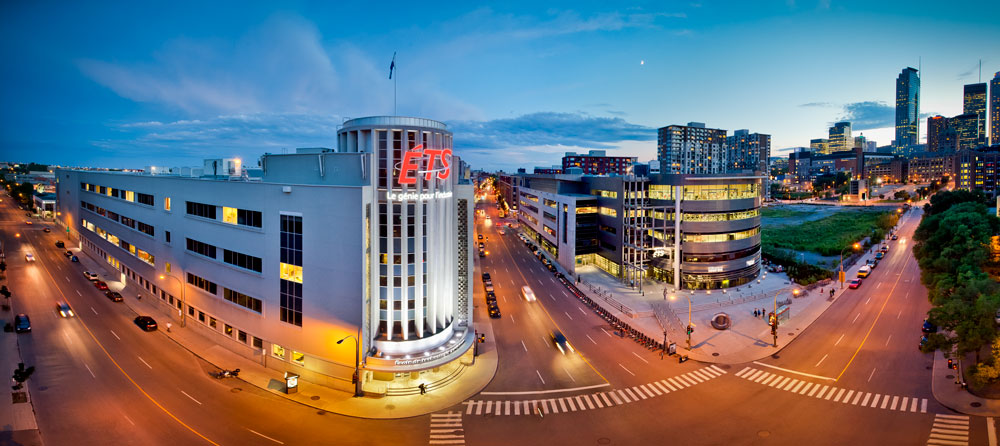
\includegraphics[width=0.47\linewidth]{Figures/vueEts.jpg}
%	}\hspace{0.009\linewidth}
%	\subfloat[second figure]{
%		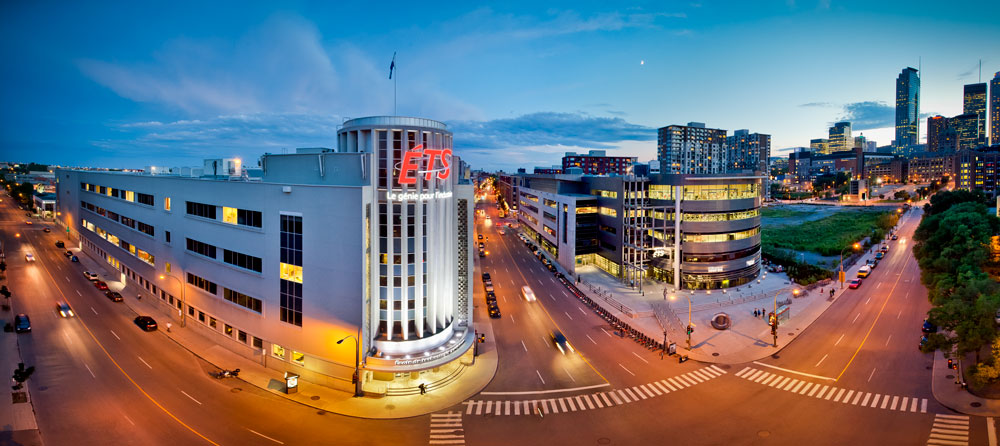
\includegraphics[width=0.47\linewidth]{Figures/vueEts.jpg}
%	}
%	
%	\subfloat[third figure]{
%		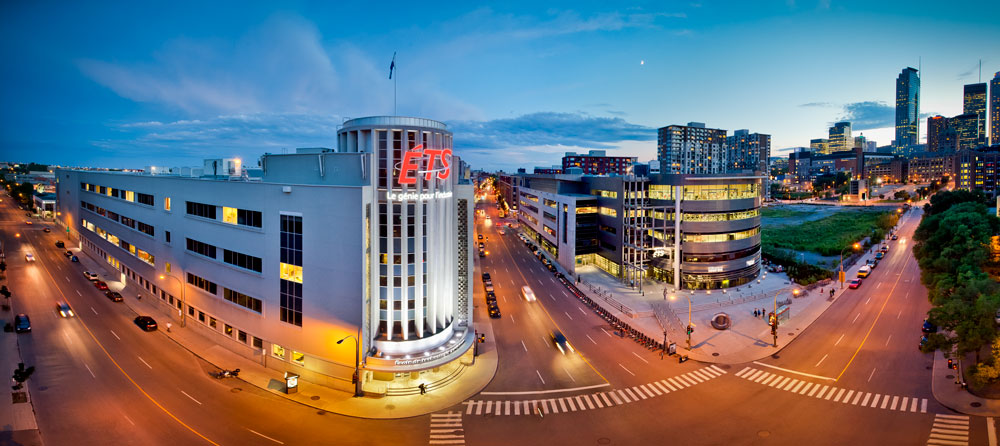
\includegraphics[width=0.47\linewidth]{Figures/vueEts.jpg}
%	}\hspace{0.009\linewidth}
%	\subfloat[fourth figure]{
%		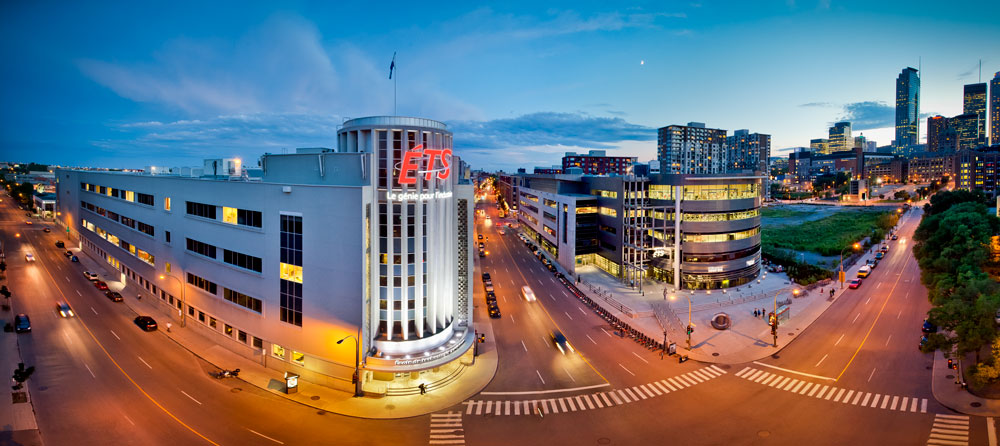
\includegraphics[width=0.47\linewidth]{Figures/vueEts.jpg}
%	}}}
%	\\ \parbox{0.975\linewidth}{\caption{Subfig example.}}
%\end{figure}
%
%In the annexes, the figures are declared in the same way. Their numbering changes automatically (e.g. Figure \ref{fig:testAp}).
%
%\subsubsection{Tables in annexes}
%
%\begin{table}
%		\parbox{0.65\textwidth}{\caption{Table in an appendix.}\label{tab:testAp}}
%
%		\begin{tabular}{|c|c|c|c|c|c|c|c|}
%		\hline
%			{\bf titre} & {\bf titre} & {\bf titre} & {\bf titre} & {\bf titre} & {\bf titre} & {\bf titre} & {\bf titre} \\
%	  \hline
%			blá & blá & blá & blá & blá & blá & blá & blá \\
%	  \hline
%			blá & blá & blá & blá & blá & blá & blá & blá \\
%	  \hline
%			blá & blá & blá & blá & blá & blá & blá & blá \\
%	  \hline
%			blá & blá & blá & blá & blá & blá & blá & blá \\
%	  \hline
%			blá & blá & blá & blá & blá & blá & blá & blá \\
%	  \hline
%			blá & blá & blá & blá & blá & blá & blá & blá \\
%	  \hline
%		\end{tabular}
%\end{table}
%
%Same behaviour for the tables (e.g., Table \ref{tab:testAp}).


%%%%%%%%%%%%%%%%%%%%%%%%%%%%%%%%%%%%%%%%%%%%%%%%%%%
% BIBLIOGRAPHY AND REFERENCES
%%%%%%%%%%%%%%%%%%%%%%%%%%%%%%%%%%%%%%%%%%%%%%%%%%%

%%- Bibliography -%%
\newpage
% Single spacing for the bibliography
\begin{spacing}{1}
	\nocite{*} % The "nocite" command can be used to print references that haven't been used in the document. The "*" option specifies that every reference should be printed
	\bibliographystyle{bibETS} % ETS bibliography style
	\addcontentsline{toc}{chapter}{BIBLIOGRAPHY} % Addition of the bibliography in the table of contents

	\bibliography{biblio_en} % List of bibliography files, biblio.bib is an example

\end{spacing}

%%- Other list of references, "refs" example --%
%%%%%%%%%%%%%%%%%%%%%%%%%%%%%%%%%%%%%%%%%%%%%%%%%%%
% IMPORTANT: HOW TO COMPILE AND PRINT ADDITIONAL REFERENCES (replace "refs" by the chosen name)
%%%%%%%%%%%%%%%%%%%%%%%%%%%%%%%%%%%%%%%%%%%%%%%%%%%
% Follow these three steps:
%   1. Compile the document once, to save the used references in refs.aux
%   2. Compile the references
% 		- On Linux: Use the "bibtex refs" command in the document folder
%		- On MacOSX (MacTex distribution): Use the "/usr/texbin/bibtex refs" command in the document folder
%		- On Windows: Edit the "update_refs.bat" script to put the right suffix ("refs" here), and launch the script
%   3. Recompile the document TWICE
%%%%%%%%%%%%%%%%%%%%%%%%%%%%%%%%%%%%%%%%%%%%%%%%%%%

\newpage
% Same commands than for the bibliography, only with the "refs" suffix
\begin{spacing}{1}
	%\nociterefs{*}
	\bibliographystylerefs{bibETS}
	\addcontentsline{toc}{chapter}{LIST OF REFERENCES}

	\bibliographyrefs{refs}

\end{spacing}

\end{document}
